\documentclass[11pt]{report}

\usepackage{url}
\usepackage{subfig}
\usepackage{tabularx}%\newcolumntype{R}{>{\raggedleft\arraybackslash}X}
%\usepackage{siunitx} % provides \SI{}{\celsius} etc.
\usepackage{etoolbox}
%\robustify\bfseries \sisetup{detect-weight = true}
\usepackage[numbers,square]{natbib}
\usepackage[affil-it]{authblk}
\usepackage{capt-of}
\usepackage{amsfonts}
\usepackage{tabularx}
\usepackage{cleveref}
\usepackage{booktabs}
\usepackage{microtype}
\usepackage{graphicx}
\usepackage{bbding}
\usepackage[noend]{algpseudocode}
\usepackage{algorithm}
\usepackage{mathrsfs}

\usepackage{balance}

\algnewcommand\algorithmicforeach{\textbf{for each}}
\algdef{S}[FOR]{ForEach}[1]{\algorithmicforeach\ #1\ \algorithmicdo} 
\def\BState{\State\hskip-\ALG@thistlm} 

\newcommand{\TRUE}{\textbf{true~}}
\newcommand{\FALSE}{\textbf{false~}}
\newcommand{\Break}{\textbf{break~}}
\newcommand{\Downto}{\textbf{down~to~}}


\newcommand\numberthis{\addtocounter{equation}{1}\tag{\theequation}}
\newcommand*\mean[1]{\bar{#1}}
\usepackage{color}
\usepackage[dvipsnames]{xcolor}

\newcommand{\commentBodo}[1]{{\color{blue}[BB thinks: {\emph{#1}}]}}
\newcommand{\etal}{et~al.}

% for table alignment
\newcommand{\Z}{\hphantom{0}}
\newcommand{\ZZ}{\hphantom{00}}
\newcommand{\ZZZ}{\hphantom{000}}
\newcommand{\ZZZZ}{\hphantom{0000}}
\newcommand{\ZZZZZ}{\hphantom{00000}}
\newcommand{\ZZZZZZ}{\hphantom{000000}}
\raggedbottom


\usepackage{color}
\newcommand{\todo}[1]{{\color{blue}[[TODO: {\emph{#1}}]]}}
\newcommand{\hopefully}{{\color{green}Hopefully: }}
\newcommand{\dave}[1]{{\color{green}[[Dave: {\emph{#1}}]]}}
\newcommand{\todoVthree}[1]{{\color{red}[[Bodo: {\emph{#1}}]]}}
\newcommand{\todoVfour}[1]{{\color{red}[[Thoughts: {\emph{#1}}]]}}
\newcommand{\todoVfive}[1]{{\color{magenta}[[Musings: {\emph{#1}}]]}}
\newcommand{\todoVsix}[1]{{\color{cyan}[[Ruminations: {\emph{#1}}]]}}
\newcommand{\LB}{\textsc{List building~}}
\newcommand{\LT}{\textsc{List traversal~}}
\newcommand{\script}[1]{$\mathcal{#1}$}



\newcommand{\GHRepo}{\url{https://github.com/Microsoft/SynthaCorpus/}}
\newcommand{\TRECAP}{TREC-AP}
\newcommand{\TopQ}{Popular queries}
\newcommand{\classificationPaper}{Song lyrics}
\newcommand{\Wikipedia}{Wikipedia titles}
\newcommand{\AcademicID}{Academic paper titles}
\newcommand{\clueWebTitles}{ClueWeb12 titles}
\newcommand{\clueWebBodiesLarge}{ClueWeb12 bodies}
\newcommand{\Tweets}{Tweets}
\newcommand{\IndriWT}{Indri-WT10g}

\newcommand{\numcolls}{nine}

\newcommand{\PP}{Imagefiles}

\title{Simulation of IR test collections}
\author{David Hawking,
Bodo Billerbeck,
Nick Craswell, and 
Paul Thomas\\
Microsoft\\
\small \texttt{david.hawking@acm.org}, \texttt{\{bodob,nickcr,pathom\}@microsoft.com}
}

\begin{document}
\maketitle{}

\tableofcontents

\begin{abstract}
Simulated test collections may find application in situations where real
datasets cannot easily be accessed due to confidentiality concerns or
practical inconvenience.  They can potentially support IR
experimentation, tuning, validation, performance prediction and
hardware sizing.  Naturally, the accuracy and usefulness of results
obtained from a simulation depend upon the fidelity and generality of
the models which underpin it.

We present and analyse a range of models for each of: document length
distribution, word frequency distribution (for independent and
non-independent cases), word length and textual representation,
generation of corpus-compatible queries, and corpus growth.  We
present results of emulating existing corpora and for scaling up
corpora by two orders of magnitude.  We show that simulated
collections generated with relatively simple methods are suitable for
some purposes and can be generated very quickly.  Indeed it is
feasible to embed a simple lightweight corpus generator into an
indexer for the purpose of efficiency studies.

The methods described here have mostly been implemented in the open source
project SynthaCorpus, accessible at:
\begin{quote}
  \GHRepo{}
\end{quote}

The tools in
SynthaCorpus assume large RAM configurations, reflecting our interest
in efficient use of large-memory machines.

\textbf{Limitations:} We restrict ourselves to the simulation of
an unstructured corpus of plain text documents.  Ideally, a generator
would also model document structure, hyperlinks, authorship, creation
dates, attachments, and file system organization.

A more basic
limitation is that our methods do not generate realistic natural language
structures, and cannot support work in translation or natural language
understanding.

\end{abstract}

\chapter{Introduction}   %%%%%%%%%%%%%%% Chap. 1 %%%%%%%%%%%%%%%%

There are a number of real world applications in which it is useful to
generate an artificial text corpus with a corresponding set of test
queries. A prime example is when a cloud hosting company (like
Microsoft) builds search
systems for hosted clients whose data is private and/or confidential.
The hosting company wishes to measure and improve indexing performance
and query processing latency and throughput, to tune a ranking
function, and to experiment with auxilliary features such as query
suggestion and spelling correction, \textit{without its employees
  having access to client documents or queries}.  If privacy and
confidentiality constraints allow an automated agent to extract
sufficient properties of a client's data then the hosting company can
build a simulated collection and work with it.

For academic research, simulated corpora can permit exact
reproducibility of efficiency experiments and meaningful study of the
scalability of retrieval systems.  A corpus can be shared exactly with
other researchers by communicating at most a few kilobytes of
parameters, while completely eliminating confounds due to differences
in tokenization and other lexical issues.  Furthermore, a
parameterized collection generator allows data sets to be engineered
to specification, permitting focused study of specific efficiency or
effectiveness factors.  Finally, a comprehensive generative model
also models the growth of a corpus, allowing retrieval systems to be
tested on data sets as they might become in the future.

In this work we report a quite thorough study of many aspects of the
collection simulation problem.  We study the properties of \numcolls~
different corpora and discuss alternative generative models for:
document length distribution; word frequency distribution assuming
independence; word dependence; and generation of the textual
representation of words.  We have developed a set of open source tools
(SynthaCorpus) for extracting properties from an existing corpus  and
for generating parameterized corpora using multiple alternative models.
We compare the properties of corpora emulated using SynthaCorpus tools
with those of the corresponding originals.

In order to build models of corpus growth we study samples of the \numcolls~
corpora and plot changes in properties as the samples grow from 1\% to
100\% of the parent.  Then, starting with a static model of the smallest
sample and modifying it according to a growth model, we generate a
corpus 100 times larger and show that its properties are quite similar
to the original.  The growth in vocabulary as corpus size
increases, as described by Herdan and Heaps, prevents us from using
the original corpus vocabulary when scaling up, even when the original
data is public.

Azzopardi et
al.~\cite{AzzopardideRijke2006}\cite{AzzopardideRijkeBalog2007} propose methods for generating known item queries
from a collection. In order to permit the study of query processing
efficiency and effectiveness
over artificially generated corpora, SynthaCorpus implements a version of Azzopardi's
best-performing method.   It also provides a facility for converting a
real query log corresponding to a real corpus, into an emulated query
log for an emulated version of the real corpus.

It is not exactly known which properties of a corpus have the greatest
influence on efficiency and observed effectiveness of a retrieval
system.  Indeed, the relative importance of the properties likely depends on
both the algorithm and the characteristics of the hardware
architecture.  A thorough study of these dependencies is beyond the
scope of the present work, but for illustrative purposes we compare
indexing and query processing rates of Indri over a tokenized form of
WT10g with those for an emulated version.

A real corpus can be emulated with different degrees of
fidelity.  It may be impractical to faithfully emulate a corpus either
due to the cost of generation or due to potential leakage of
private information.  Our study sheds light on the range
of degrees of fidelity and the costs of achieving a specified level.

\section{Text generation as encryption}
Possibly the simplest method for emulating a corpus \script{C} is to
encrypt it using a substitution cypher.  If we used a fixed
word-for-word substitution, each word in \script{C} would be replaced
by the corresponding word in a parallel vocabulary.  The parallel
vocabulary could be a permutation of the original, a vocabulary of
equal or greater size from a different corpus, or a list of made-up
words. 

This simple method has the advantage that all the characteristics of
\script{C} can be preserved, including length, structure, punctuation, links
and metadata.  Encryption code requires a large mapping table
between the vocabularies, but can be very fast.

On the downside, a determined adversary Eve may be able to extract
useful information out of the emulated corpus \script{E}. Furthermore,
the method is constrained to emulation of an original corpus.  It is
not feasible to create a scaled-up emulation of \script{C}, nor to
create a distribution of corpora with very similar properties to
\script{C}, nor to engineer a corpus to have specified properties.

Our interest is in generating corpora in all those scenarios, but we
may return to the \textsc{substitution} algorithm later in the monograph.


\section{Simple language models for text generation}
Generative language models used in IR are 
typically used to assess the likelihood that a document and a query
were generated from the same model, rather than to actually generate
text.  They could, however, be used for synthetic corpus generation,
as illustrated in the simple-minded algorithm \textsc{baseline}:  


\todo{Probably should recast the following as an algorithmic environment}
\begin{enumerate}
\item Extract a unigram language model (LM) from a real corpus \script{C}, 
representing the language model as a cumulative probability histogram,
in which observed words ($x$-axis) are ranked by descending probability.
(Zipfian model. \cite{zipf1949humanBehaviour})

\item Repeat the following until the desired amount of text has been generated:
\begin{enumerate}
\item Generate a pseudo random document length $l$ (in words) from a
  length distribution derived from \script{C}.
\item Generate $l$ uniformly distributed random numbers in the range 
  $0\ldots1$.  Use the cumulative
  probability histogram to map each of them to a word and emit that word.
\item Emit a document boundary marker.
\end{enumerate}
\end{enumerate}

We present the \textsc{baseline} algorithm to illustrate the general
idea of corpus emulation, and to illustrate the shortcomings of such a
straightforward approach.  Ideally, the resulting corpus \script{E}
should closely match the modeled properties of the 
original corpus but \textsc{baseline} suffers from a number of limitations:
\begin{enumerate}
\item Because we are sampling ``with replacement'' the expected vocabulary size
  of \script{E} will be less than that of \script{C} since some words
  will likely not be sampled.
\item Words are generated independently.  Phrase and sentence
  structure are not modeled and nor is the tendency of word
  occurences to cluster in documents.
\item The vocabulary of the synthetic corpus cannot be larger than
  that of the emulated one.  Words not found in the base corpus cannot be
  emitted.  That means that scaling \script{E} beyond the size of
  \script{C} will result in decreasing
  fidelity since laws due to Herdan \cite{Herdan1960} and Heaps
  \cite{Heapslaw1978} tell us that
  the vocabulary size of a real corpus should grow with the size of the text.
  Williams and Zobel \cite{williams2005searchable} have confirmed this
  growth in much larger datasets than available to earlier authors.
\end{enumerate}

We will see later on how to overcome these limitations.

Note that the size of a language model (probability histogram) may be
large.  A very large corpus may contain hundreds of millions of
distinct words.

We present some experimental results for \textsc{baseline} in
Section \ref{baseline_expts}.  Naturally, the range of applications for a
synthetic corpus can be increased if more sophisticated modeling is
undertaken.  A number of more sophisticated generative models are
available.

\section{More sophisticated models}

\todo{table with models (plus corpus), qualities - fill in with
  ticks/crosses.   even better, a table with real numbers (e.g. vocab
  size).  The ticks and crosses  table could go in the
  introduction. But the real numbers part should go in the empirical
  chapters 9-14, probably Ch 10.}
\todo{Perhaps we could each take one method from this section and run
  it to generate… something… for comparison.  --> Chapter 10}

\textit{Topic modeling via Latent Dirichlet Allocation} can be used to
better model the tendency of subject words to
cluster~\cite{blei2003latent}.  Separate LMs are generated for topics
represented in a corpus and documents are generated as a mixture of a
subset of topics.  For instance, Wallach et
al.~\cite{wallach2009evaluation} propose a method to generate held-out
documents given the remainder of a collection.

\textit{$n$-gram language models} can at least partly model the natural language
structure of real text.   A corpus may be modeled as a mixture of 
unigrams and higher-order ``grams''.  
While taking $n$-grams into account has been shown to be useful (see
e.g.~Bendersky et al.~\cite{bendersky2010learning}), unsurprisingly 
there is little prior work on
generating text corpora using $n$-grams alone.

\textit{Markov chains.}  Sequences of words in natural language text
could in theory be modeled using a Markov chain \cite{KemenySnell1960}
but with vocabulary sizes in the hundreds of millions, the size of
the transition probability matrix and the effort required to calculate
it would be prohibitively large.

\textit{Recurrent neural nets (RNNs)} have been used to
model language structure even more accurately, by modeling longer
range dependencies.  Sutskever et~al.~\cite{sutskeverMartensHinton2011generatingTraffic} have
demonstrated how this technique can, with appropriate training data,
generate fragments of text which convincingly match the style of
e.g.~Shakespeare or a technical report.  The resulting text conveys no
real meaning but presents groups of words in plausible order, and with
plausible punctuation.
\todo{Run Sutskever et al - does a Shakespeare-sized generated corpus
  have same tf/df distribution as real Shakespeare? Other properties e.g. vocab size
	NB this (df/tf) is a general problem when sampling from a
        histogram w/rare terms
        - rare terms won't appear "enough"  --> Chapter 10}


\textit{Natural language generation from real world semantics}, that is,
the generation of artificial text which conveys real meaning, seems at
this point in time to be restricted to narrow semantic domains such as
sportscasting, e.g.~\cite{ChenKimMooney2010}.

Most applications in the ``experimenting with private data'' area would require 
sophisticated models like these, but are constrained by the need to maintain
security of private and confidential information.  A very accurate
model might enable the deduction of confidential information.  For
example a sophisticated model may allow an attacker to determine that
the sentence, ``Our company will acquire company X'' has higher
probability than the sentence, ``Our company will not acquire company X''.
It remains to be seen whether a useful balance can be struck between
representational fidelity and preservation of privacy.

The more sophisticated models listed above remove
the need to assume word independence but still require large models,
are still limited to a fixed vocabulary, may require more CPU time 
to generate words, 
and generally require more effort in model generation.  Chapters
\ref{chap:dependenceExpts} and \ref{chap:speed} provide some empirical
data on this.

For efficiency and scalability experimentation there are practical
advantages in overcoming these limitations, even if the modeling 
is less faithful to natural text.  Overcoming the limit of fixed 
vocabulary seems critical to scalability experimentation; smaller
models allow easier sharing of experimental data with colleagues;
and efficient generation of text enables faster experimental
turn-around times.    

\section{Efficiency and scalability}
 
Studies of the efficiency of text indexing algorithms
have often reported time and space results for the indexing of a single
corpus (such as GOV2 \cite{ClarkeCS2004}), e.g.~\cite{KonowNCL2013},
\cite{DingAS2010} and many referenced in \cite{ZobelMoffat2006}.
Empirically assessing the scalability of
algorithms is difficult because of heterogeneity between corpora of 
different sizes.  The data size of one corpus may be $x$ times larger than 
that of another but the ratio of the magnitude of the indexing
tasks may be very different from $x$ due to different vocabulary sizes, 
different word frequency distributions, and different proportions of
indexable text.

Another limitation of indexing efficiency studies is that published
results are difficult to reproduce because of differences in details
of how each indexer scans text.  Indexers differ widely in the
following aspects: recognition and conversion of character sets;
stopword handling; word-break characters; stemming; parsing of markup;
recognition and handling of text in ``fields''; handling of comments
and no-index sections, obedience to `robots' metatags; indexing of
element attributes; recognition of XML entities; and handling of mark-up
which isn't well-formed.



There is now considerable interest in the study of memory-resident
indexing and retrieval algorithms for NUMA (Non-Uniform Memory Access)
architectures.  Since 2010 or so, it has been possible to purchase
off-the-shelf servers configured with multiple terabytes of RAM. Such
servers are characterized by great variations in memory access speed,
due to multiple levels of cache, to the need to maintain cache
coherency, and to the closer association of banks of RAM to just one
of several CPU chips.  For example, the best access latency in clock
cycles for different levels of memory in the Intel Core i7 Xeon 5500
series is 4 for L1 cache, 10 for L2 cache, 40 for L3 cache, 60 for
local DRAM and 100 for remote
DRAM.\footnote{\url{https://software.intel.com/en-us/forums/intel-manycore-testing-lab/topic/287236}
  accessed 07 Jan 2016.}

Meaningful empirical comparison of retrieval algorithms in NUMA
environments requires large corpora, which are difficult to share with
others -- test collections like ClueWeb09 have been shared in the past
by the
cumbersome means of shipping arrays of hard disks.

\begin{table*}[t] \tiny
\caption{Details of the corpora used in sampling
  experiments.\label{t:corpora}  $N$ - Number of documents in the
  corpus; $|V|$ - number of distinct words in the vocabulary; $P$ -
  Total number of word occurrences (postings.)
}
%   \sisetup{
%        detect-mode,
%        %table-format=.,
%        input-open-uncertainty  = ,
%        input-close-uncertainty = ,
%        table-align-text-pre    = false,
%        table-space-text-pre    = (,
%        table-space-text-post   = ),
%        group-separator = {,},
%        input-decimal-markers={.},
%        }
\begin{tabular}{lrrrl}%{\linewidth}{lS[table-format=1.2]@{}S[table-format=1.2]@{}S[table-format=1.1]@{}l}
Name                 & \multicolumn{1}{c}{$N$} & \multicolumn{1}{c}{$|V|$} & \multicolumn{1}{c}{$P$} & Remarks\\
\hline
\TRECAP              &   0.24M &   0.29M &  100.1M & TREC newswire covering 24 months\\
\TopQ                & 100.00M &   6.41M &  381.0M & popular Web queries\\
\classificationPaper &  27.92M &   0.91M &  153.0M & song lyric lines\\
\Wikipedia           &  11.06M &   2.32M &   32.7M & Wikipedia titles (inc.~redirects)\\
\AcademicID          &  89.53M &  11.98M & 1003.6M & collection of paper titles\\
\clueWebTitles       & 728.88M &  21.78M & 5687.3M & ClueWeb12 document titles\\
\clueWebBodiesLarge  &  23.30M &  61.11M & 5340.1M & subset of ClueWeb12 bodies\\
\Tweets              & 710.62M & 340.75M & 8843.7M & daily Twitter samples covering 18 months\\
\IndriWT             &   1.94M &   5.65M & 1040.1M & TREC WT10g words extracted by Indri\\
\hline
\end{tabular}
\end{table*}

Logically, a synthetic corpus derived from a real one may be
considered to be a highly compressed version of the original.  Instead
of shipping hard disks of text data we can ship a much smaller
model plus a small set of parameters, a random seed, and give access
to the generator code (e.g. \textsc{SynthaCorpus}).

The compression factor can be increased significantly if we generate the word
representations, and mathematically model the word probability
distribution rather than recording a full histogram.  In the \textsc{baseline} algorithm
presented earlier, if the random number generator picks say word 13507, then
we look up the word table in the language model and find that that 
corresponds to ``adumbrate''.  If we instead generate the word
representations, then an algorithm maps word number 13507 to a unique
sequence of characters rather than to a known word.  For example, it
may generate ``xx\$p2''.  Note that a word representation generator
may be
needed to solve a limitation mentioned above -- that scaling up a
corpus should not assume a fixed vocabulary.

A generator for word representations opens another exciting
possibility.  With such a generator we may never need to physically
instantiate the corpus.  Instead, the word generation could be done
internally to the indexer, avoiding the need to store text on disk and
to read it during indexing.  We call this \textit{on-the-fly generation}.
For on-the-fly generation to be practical, the random selection
of the word number and the generation of its character representation,
must require minimal memory to avoid interfering too much
 with use of memory
caches by the indexing algorithm being studied.  It should also
take no more CPU time than would be used by reading and parsing
a word from the real collection on a hard disk drive.  These
constraints limit the sophistication of the methods used in on-the-fly
generation. 

Synthetic corpora, whether instantiated or not, can be used
for studies of efficiency and scalability of indexing algorithms.
Combined with simulated known-item queries or emulated query logs
synthetic corpora can potentially also be used to study the efficiency
of query processing algorithms.  Indeed, since known item queries
provide for limited evaluation without the need for human judgments, 
it is possible to simulate test collections and to use them to compare
and tune retrieval methods.

\section{Outline of the monograph}
In this paper we study the \numcolls~ different base corpora documented in 
Table \ref{t:corpora}.  The selection of these corpora
 reflects an interest on our
part in indexing and querying large numbers of short texts such as
tweets. However, \TRECAP~is a TREC corpus comprising the full text of
the AP newswire articles, and \clueWebBodiesLarge~comprises the 
extracted full text of 20 million ClueWeb12 documents.  A third 
collection of longer documents is \IndriWT.  It comprises the 
document boundaries and indexable tokens extracted by the 
Indri\footnote{\url{http://www.lemurproject.org/indri/}}
retrieval system from the well-known WT10g TREC corpus. We
created it to permit fair comparison of indexing and retrieval runs over base and
emulated versions of the same corpus.

We focus on emulating the following corpus characteristics:
\begin{enumerate}
\item Number of documents.
\item Document length distribution.   
\item Total number of word occurrences (postings) $P$.  This is the main
  determinant of the scale of an indexing task.
\item Vocabulary size $|V|$.  This determines the size of the word
  dictionary and influences the time taken by word insertions and
  lookups.
\item Word probability distribution.  This determines the distribution
  of postings list lengths and the length of the longest postings
  list.  The best choice of index data structures and algorithms may 
  depend upon this. 
\item Word dependence.  We try to capture the tendency of certain
  pairs of words to associate within documents, the tendency of
  certain words to appear more often in particular documents than
  would be expected by chance, and the tendency of certain word
  $n$-grams to appear more often than would be expected by chance.
  At the time of writing the \textsc{SynthaCorpus} code is able to model
  $n$-grams only.  However, we present algorithms for modeling word
  burstiness and word co-occurrence.
\item Characteristics of word representations.  The length of words
  and the patterns of characters in the representation may affect 
  hash table collision rates or the efficiency of tree structures.
\item The tendency (\cite{zipf1935psycho}) of short words to
  occur more frequently than long ones.
\end{enumerate}

In Chapter \ref{LenMod} we consider a range of models for document 
length distribution. In Chapter \ref{TProbModInd} we explore models of
word probability distribution, assuming independence.  In Chapter
\ref{TDepMod} we look at dependence models, and the important question
of how to measure whether the associations between terms have been
properly modeled.  Chapter \ref{TermReps} discusses the generation of
sequences of characters to represent words, when it is not possible to
use the lexicon of a corpus being emulated.  In Chapter
\ref{GrowthModels} we show how the characteristics of
samples of each corpus change as we increase the size of the samples
from 1\% up to 100\%.  From these observations we derive growth
models. Chapter \ref{QGen}
discusses methods for generating corpus-compatible queries and
judgments, and also for simulating query logs.

Chapter \ref{chap:SynEval} outlines approaches to evaluating the quality of
synthetic test collections, and Chapter \ref{chap:speed} measures the speed
of generation of text corpora and of known-item query sets.

In Chapter \ref{EmExpts} we attempt to emulate each corpus \script{C},
by modeling the properties listed above, and using models, including
\textsc{baseline} , to control the generation of an emulated corpus
\script{E}.  We compare the properties of \script{E} and \script{C}
and conclude that, for the best type of model, they are sufficiently
similar to at least permit their use in efficiency studies.  Chapter
\ref{chap:dependenceExpts} experiments with 2-gram generation. Chapter
\ref{chap:wordRepExpts} empirically compares methods for generating
artificial words.
Chapter \ref{SUExpts} describes scaling-up experiments which attempt
to emulate \script{C} from the average properties of a number of 1\%
samples of \script{C}.  Fidelity is less than in the direct emulation
case, but the results are still quite promising.

Chapter \ref{chap:practicalities} discusses practical issues and trade-offs in
test collection simulation, and the possibilities and limitations of
on-the-fly generation.   Chapter \ref{RelatedWork} reviews related
work.

In the Information Retrieval field it is common to use the term
``term'' to refer to words.  Here we also use it to refer to compounds
such as $n$-grams.  When we are specifically talking about words, we
use the word ``word'' rather than the term ``term''.


\chapter{Modeling document lengths}   %%%%%%%%%%%%% Chap. 2 %%%%%%%%%%%%%
\label{LenMod}
In many applications, approximate modeling of the distribution of
document lengths will suffice.  However, there are scenarios in which 
accurate modeling is desirable.  For example, the efficiency of some indexing or query 
processing algorithms may be affected by very long or very short
documents.  Furthermore, distributions of term cooccurrences,
distributions of TFs, and topic mixtures are all affected by the
distribution of document lengths.

We have undertaken a study of a number of different document length models.  In the
following, the length of a document is defined as the number of
indexable words it contains.


\section{Left-truncated Gaussian length model}
The mean and standard deviation of document lengths in the primary corpus are easily
calculated. We can then sample lengths from a normal distribution
with those parameters using an appropriate function such as ceil() to convert real
values to integer lengths.  If a zero or negative length is sampled
it is rejected, leading to a shift in the actual mean of the truncated
distribution. We applied simple multiplicative correction factors to
both mean and standard deviation to more accurately model the primary
corpus.

Efficient generation of normally distributed random numbers is 
possible using the method of Marsaglia and Bray \cite{Marsaglia1964}.

We found that for many corpora the truncated normal distribution significantly
under-generates longer documents found in the original distribution.
Furthermore, we see no theoretical reason to expect that document
lengths
ought to be normally distributed.  Therefore, apart from
implementation convenience, there is little to recommend this model.

\section{Negative binomial length model}
If we added a symbol representing end-of-document to our word
distribution and emitted it with fixed probability $p$, then each act
of sampling would constitute a Bernoulli trial in which the emission
of an end-of-document symbol represents the ``failure''.  In this
scheme, the number of successes (i.e. length of document in words)
before a failure would be distributed according to a negative
binomial.

Unfortunately, the form of negative binomial which fits actual
document length distributions best, tends to be one for multiple
failures.  Even if we interpret the additional symbol as a
possible-end-of-document, it is hard to suggest a good reason why
document authors would stop at the $k$-th of the possible
stopping points.

Although the negative binomial has some relation to a plausible author
model, it's ability to fit observed data is less good than that of the
gamma distribution.

\section{Gamma distribution length model}
A gamma distribution can be specified using two real parameters, shape
and scale.  Depending upon the values of these parameters the form of
the distribution can approximate normal, exponential, uniform and
other forms.  This flexibility allows gamma to model observed length
distributions for many real corpora with greater fidelity than was the
case with the two preceding models.  Unlike the Gaussian, gamma can
emulate the heavy tail found in many observed document length
distributions.

We estimated the parameters for a gamma distribution using the method
and code due to Minka \etal~
\cite{Minka2002,InferNET14}\footnote{Downloadable from
  \url{http://infernet.azurewebsites.net/}. (Microsoft.Infer.Distributions)}.
We implemented sampling from
a specified Gamma distribution using the efficient method of Marsaglia
and Tsang \cite{MarsagliaTsangGamma2000}.

The gamma distribution can achieve good fidelity on some corpora,
requires only two parameters, and can easily control the generation of
a corpus much larger than the original.  Unfortunately, the gamma
distribution, like the Gaussian and negative binomial, is unable to
model actual distributions with multiple points of inflection. Such
distributions seem to be reasonably common and may correspond to
corpora consisting of a mixture of document types.  E.g. a mixture of
abstracts and articles.

Simple mathematical models capable of fitting the distribution of
document lengths in arbitrary corpora being difficult to find, we
investigated piecewise linear models.

\section{Piecewise linear length model}
Initial experiments with piecewise segments defined as either fixed
intervals on the horizontal axis or fixed areas under the curve were
unsatisfactory.  Fine segments were needed to model perturbations in
the curve resulting in large models.  

We next tried an adaptive method.  We bucketed document lengths and
started with a single segment extending from the first bucket to the
last.  We then recursively split it at the bucket where the deviation
of actual frequency from the predicted by the line segment was at a
maximum, provided that deviation was larger than a threshold.

This method was capable of modeling multi-modal distributions but
again encountered problems with certain corpora.  We were unable to
find a combination of bucket size and split threshold which achieved
sufficient modeling accuracy on all the corpora while using only a
modest number of segments.  Small bucket sizes were needed to model
narrow peaks but led to jitter and large numbers of segments.

Given that the piecewise linear model provides no explanatory power, relies on
heuristics, and requires a relatively large number of parameters to achieve 
good results across corpora, we proceeded to investigate using the actual histogram of
observed lengths, bucketed and/or scaled up as necessary.
 
\section{Length models relying on observed histograms}
A histogram of observed document lengths for an original corpus is often
reasonably compact, even with a bucket size of 1.  When emulating the
corpus we could generate document lengths by traversing the histogram,
first generating all the documents of length 1, then all those of
length 2, and so on up to the maximum observed length.   This would be
perfectly acceptable if we were able to assume that the order of
occurrence of document lengths was arbitrary and had no effect on
anything we wanted to measure or observe on the emulated data.

If this were not the case, we could expand the histogram into an
array of lengths, in which each length occurs with the frequency
shown in the histogram, and shuffle it.  An in-place random shuffling algorithm
due to Durstenfield \cite{Durstenfeld1964}\footnote{It is a more
  efficient version of the Fisher-Yates method and is also known as
  Knuth shuffle.} runs in linear time.  Shuffling is equivalent to
sampling from the histogram without replacement.

If the number of distinct document lengths is high then it may be
necessary to use a larger bucket size.  When the histogram expansion
process is expanding a bucket, the lengths chosen could be uniformly sampled from the
range of lengths represented by the bucket or perhaps a fixed
representative length could be emitted.   There would be advantage to
using a dynamic bucket sizing scheme which uses narrow buckets for the
shorter lengths where accurate modeling may be more important and
increases them in arithmetic, geometric or other sequence.

Scaling up a histogram in order to generate a corpus larger (or
smaller) than the original is easily achieved by multiplying the
bucket counts by a constant factor.

Perfect fidelity can be achieved when emulation uses an unscaled,
unbucketed length histogram from the original corpus. A limitation
when scaling up is that without some sort of smoothing, there is no
possibility of generating lengths which were not observed in the
original corpus.

\section{Length models: which to choose?}

\begin{figure}[p]
\label{figure-docLengthFitting}
    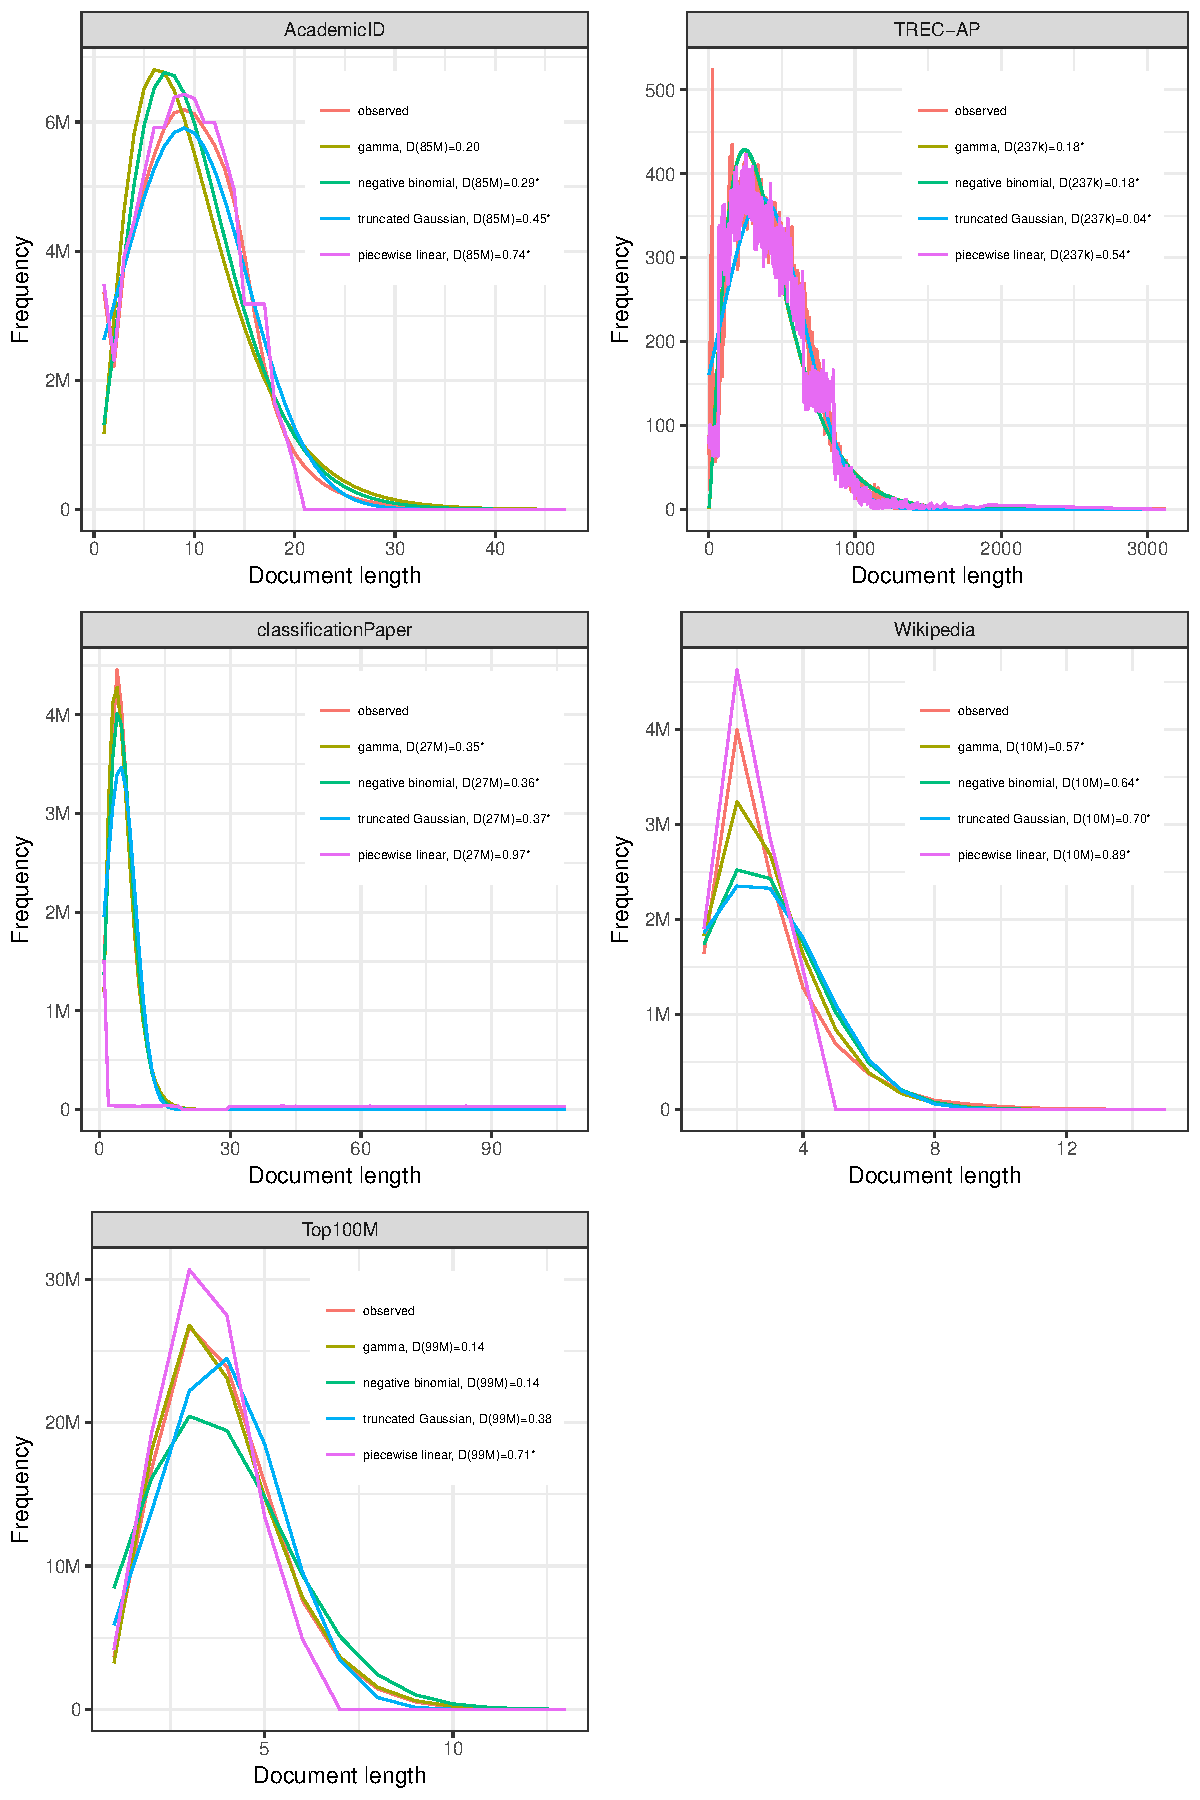
\includegraphics[width=0.8951\linewidth]{plots-pathom/doclenhist/doclen-dists.pdf}
\caption{Different document length models applied to
  five of the nine corpora.  The Kolmogorov-Smirnov tests has been
  used to compare each model to the observed distribution.  Values of
  the KS statistic are shown (smaller is better).  In each of the five
cases, the gamma distribution performs as well or better than the
other models.}
\end{figure}  

\todo{Tabulate the model sizes for each of the methods.}
\todo{Paul: •	Each of the models in §3.1, 3.2, … could be illustrated with examples of the resulting fit, i.e. a pointer into the table we’ve been building. That table could easily be extended to include the total storage needed for each model (or model/seed-corpus pair).}

Figure \ref{figure-docLengthFitting} presents the document length
distributions for several of the nine corpora and shows how well they
can be modeled by the approaches discussed in this chapter.

We recommend choosing the gamma model if mathematical simplicity and a
small number of parameters is desired, unless the observed length
distribution for the primary corpus is clearly multi-modal.  It would
be possible to model a distribution as a mixture of gamma
distributions, but the complexity of doing this would reduce the
advantage and argue for a histogram-based approach.

In other circumstances, the use of a histogram-based method is
preferred despite being a highly-overfitted model. The optimal
bucketing scheme and whether to implement some form of smoothing
should be determined after analysis of the data.




\chapter{Modeling word frequencies, assuming independence} %%%%%%%%%%%%% Chap. 3 %%%%%%%%%%%%%
\label{TProbModInd}



We start by exploring the use of the full language model and the 
\textsc{baseline} algorithm and move on to a model which is 
considerably more sophisticated, though it still assumes word
independence.

\section{Generating words with the simple-minded algorithm}
\label{baseline_expts}

\begin{table}[ht]
\centering
\caption{Emulation of \AcademicID~corpus using the \textsc{baseline}
  algorithm. \label{t:baseline}}
\begin{tabular}{lrrr}
\hline
Corpus & $P$ & $|V|$ & singletons\\
\hline
\script{C}            & 1004M  & 11.98M & 7.187M\\
\script{E}$_{10\%}$   & 100.4M & 2.715M & 1.676M\\
\script{E}$_{100\%}$  & 1004M  & 9.053M & 3.256M\\
\script{E}$_{1000\%}$ & 10040M & 11.98M & 0.003M\\
\hline
\end{tabular}
\end{table}

As noted in the introduction we can use a cumulative word probability
histogram as the basis for word-id generation.  We have
done this for the \AcademicID~corpus described in Table
\ref{t:corpora}.  We used the \textsc{baseline} algorithm to generate
simulated corpora of 10\%, 100\% and 1000\% of the number of
postings in the original corpus.  The cumulative word probability
histogram was derived from the full \AcademicID~corpus.
To test that our algorithm and the underlying pseudo random number
generator (Mersenne Twister \cite{MatsumotoN1998}, Tiny 64bit version) were working
correctly
we mathematically predicted what percentage of singleton words in the
language model would fail to be selected in $P=1004$ million draws --
the number of postings in Academic paper titles. Since each draw has a
$(P-1)/P$ probability of missing a particular singleton and there are
$P$ draws, we can raise $(P-1)/P$ to the power of $P$ to get the
probability of missing a singleton entirely.  The predicted and
observed proportions of missed singletons were 0.36785 and 0.36788
respectively, showing agreement to 4 decimal places.  Part of the
small disagreement may be due to 
\textsc{baseline} missing not only singletons but also words with
higher frequency through the same process.  The net effect is a significant
overall loss of vocabulary for \script{E}$_{100\%}$.

The results for \textsc{baseline} are tabulated in Table
\ref{t:baseline}.  When simulating a corpus of the same size as
\script{C} the vocabulary size is only 76\% as large as the original.
The under-generation of the vocabulary occurs
essentially because we are sampling words from the model \textit{with replacement}.

When the number of samples drawn from the language model is increased
by a factor of ten (\script{E}$_{1000\%}$) virtually all the words are
selected.  This confirms that the random number generator has
sufficient resolution.  However, the vocabulary size can not and does
not exceed the size of the model and the number of singleton words
reduces to almost zero (because former singletons are drawn more than
once).

A better approach to emulation would involve sampling \textit{without
  replacement}.  Implemented using rejection, this might be
impractically slow, but fast implementations are possible, most
obviously using the same approach as recommended for the document
length histograms.  That is, expand the histogram into an array of
word occurrences and shuffle it using Durstenfeld's algorithm.

The model sizes for the \textsc{baseline} algorithm are large.
In the case of the \AcademicID~corpus, the size of the model is
approximately 12 million elements, each comprising a text string and
a high-precision probability value.  For the \Tweets~corpus the
corresponding figure would be more than 340 million.


\section{Mathematical modeling of word distributions.}

\begin{figure}[p]
\centering
\subfloat[][\TRECAP]{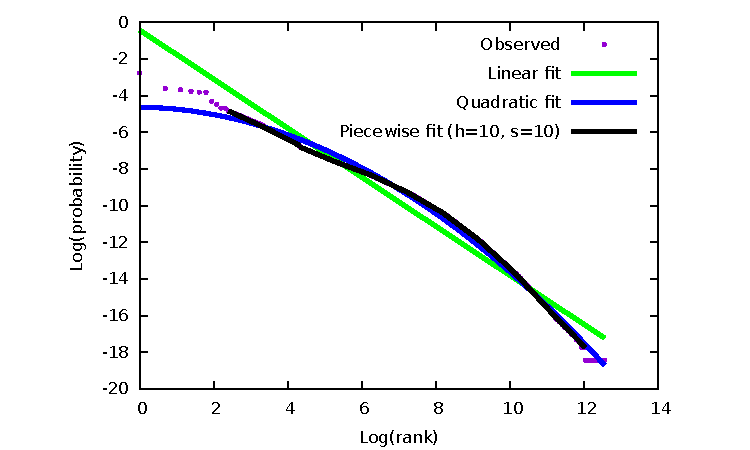
\includegraphics[width=0.705\textwidth]{\PP/LsqfitPlots/TREC-AP_lsqfit.pdf}}

\subfloat[][\IndriWT]{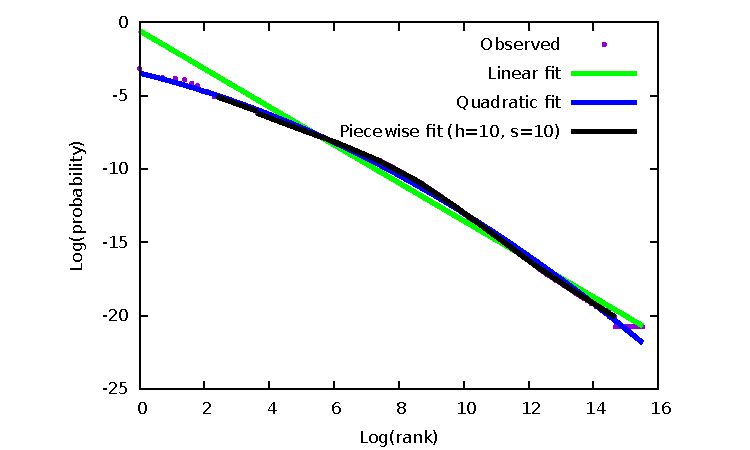
\includegraphics[width=0.705\textwidth]{\PP/LsqfitPlots/Indri-wt10g_lsqfit.pdf}}

\subfloat[][\clueWebBodiesLarge]{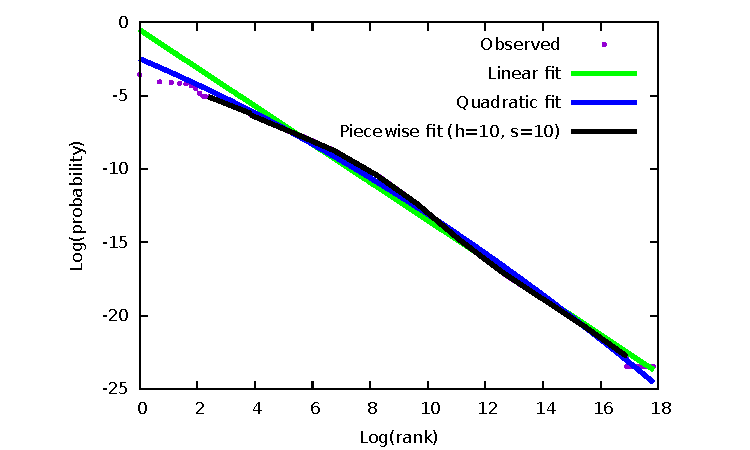
\includegraphics[width=0.705\textwidth]{\PP/LsqfitPlots/clueWeb12BodiesLarge_lsqfit.pdf}}

\caption{Word probability distributions in log-log space for three 
  real TREC-derived corpora.  Lines of linear, quadratic and piecewise
  linear fit are also shown.  
\label{fit1}}
\end{figure}


\begin{figure}[p]
\centering
\subfloat[][\TopQ]{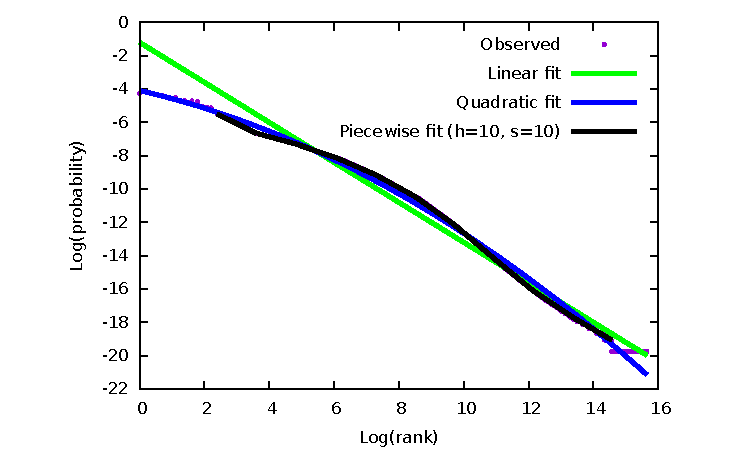
\includegraphics[width=0.705\textwidth]{\PP/LsqfitPlots/Top100M_lsqfit.pdf}}

\subfloat[][\classificationPaper]{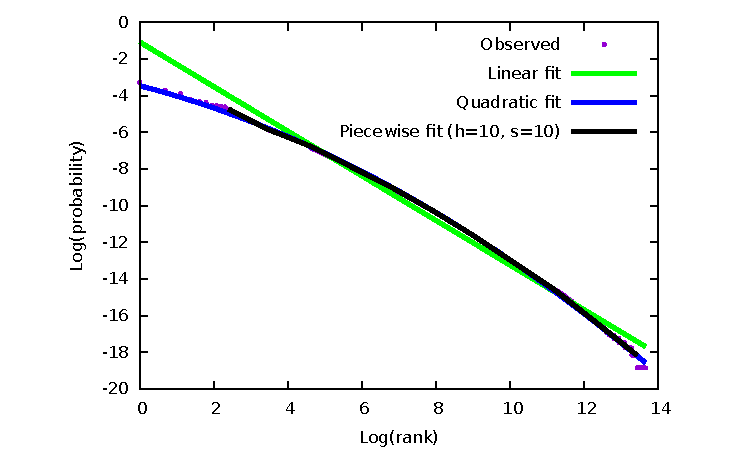
\includegraphics[width=0.705\textwidth]{\PP/LsqfitPlots/classificationPaper_lsqfit.pdf}}

\subfloat[][\Tweets]{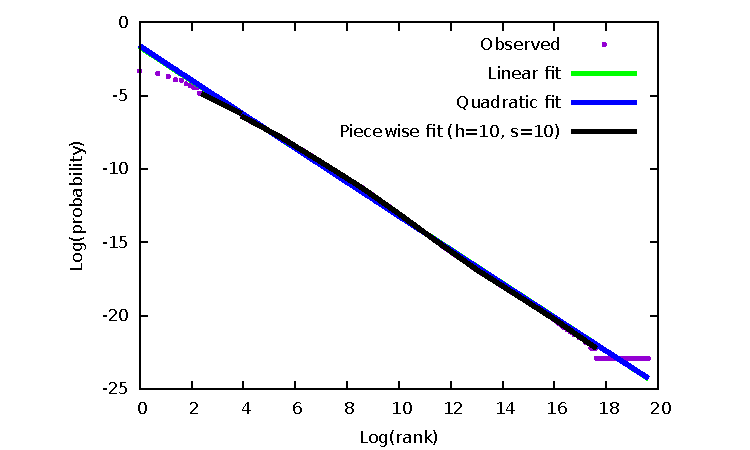
\includegraphics[width=0.705\textwidth]{\PP/LsqfitPlots/Tweets_lsqfit.pdf}}
\caption{As for the previous figure but showing three corpora
  comprising very short texts: Web search queries, song lyric lines
  and tweets.
\label{fit2}}
\end{figure}

\begin{figure}[p]
\centering

    \subfloat[][\Wikipedia]{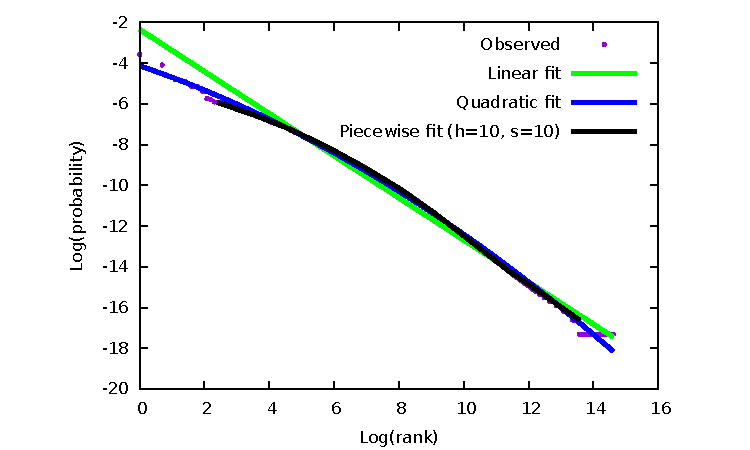
\includegraphics[width=0.705\textwidth]{\PP/LsqfitPlots/Wikipedia_lsqfit.pdf}}

    \subfloat[][\AcademicID]{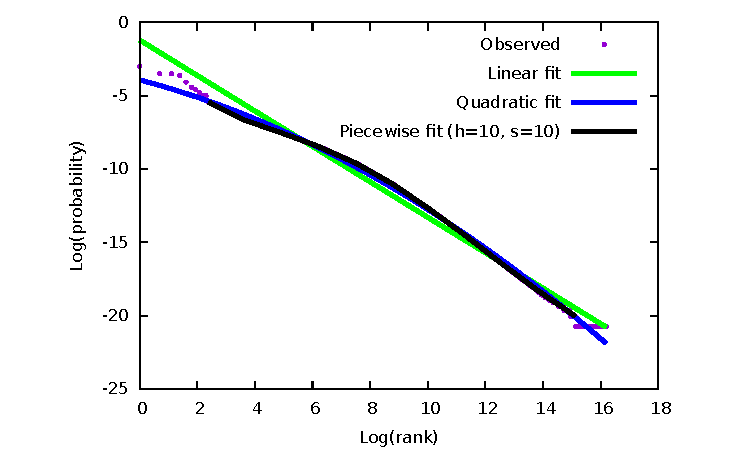
\includegraphics[width=0.705\textwidth]{\PP/LsqfitPlots/AcademicID_lsqfit.pdf}}
    
    \subfloat[][\clueWebTitles]{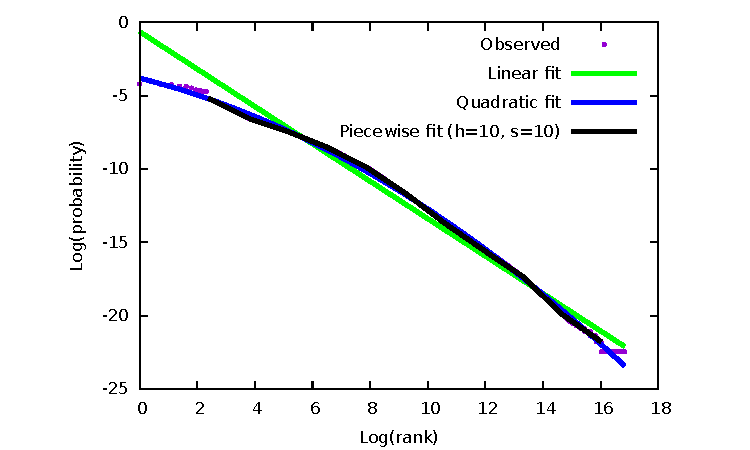
\includegraphics[width=0.705\textwidth]{\PP/LsqfitPlots/clueWeb12Titles_lsqfit.pdf}}

\caption{As for the previous two figures.  Showing three corpora
  comprising document titles from English Wikipedia, academic
  papers, and ClueWeb12 documents.
\label{fit3}}
\end{figure}



Many believe that the word probability distribution in a text corpus
follows Zipf's law \cite{zipf1949humanBehaviour}.  That law states
that the probability $Pr(t_r)$ of the $r$-th most frequent word
is proportional to a negative power $\alpha$ of the rank $r$. We can
relate this to a continuous probability function in which $r$ is real:
\[
Pr(t_r) \propto r^\alpha
\]

If this model applied perfectly, a log-log plot of probability 
against rank would show a negatively sloping straight line. However, it is
frequently observed that real-world frequency distributions
conform to Zipf's law less well at both high and the low frequencies.
Baeza-Yates \cite{baezaYates2015incrementalSamplingOfQueryLogs}
reports that singleton queries are far more heavily represented in 
query frequency distributions than would be predicted by a power law 
which fits the upper part of the distribution.

A considerable literature has accumulated describing approaches to
achieving better modeling of such ``Zipfian'' distributions.  One of
them \cite{Laherrere1996} proposes a ``parabolic fractal'' model which
would lead to a quadratic fit in log-log space.  Figures
\ref{fit1}--\ref{fit3} show log-log plots of word probability against rank along
with both linear and quadratic lines of best fit.
\todo{In Table fit make notation consistent with text.  Note
  availability or otherwise of datasets.}

Note that only a subset of points are shown -- the full number of
points is too large to display.  Least squares fitting is carried
out on the plotted subset of points.  The points in the subset were
chosen such that each point in the subset was more than a small
distance $\epsilon$ (in log-log space) away from the others.  The
number of points was thus reduced to the order of a thousand rather
than tens or hundreds of millions.  One effect of this procedure
is to reduce the bias of fitting toward the tail due to its huge
preponderance of points.

More recently Petersen \etal~\cite{PetersenSL2016} have conducted a
very comprehensive data fitting study of distributions in Information
Retrieval (IR). For nearly all of 28 different IR corpora they found
that, of 16 different models of the word frequency distribution,
the Yule-Pareto was the best fitting discrete
model and Generalized Extreme Value (GEV) the best fitting continuous
one.  In Figure 3 of their paper Petersen \etal~ graph the results of
fitting on four of the corpora.  It's interesting to note that in the
case of the iSearch and ClueWeb12 cat. B corpora their GEV line of best
fit closely matches the head section of the plot but deviates markedly
in the middle section.\footnote{Note that  Petersen \etal~ plot
  probability against word frequency rather than probability against rank.}

Even more recently Chierichetti \etal~\cite{ChierichettiKP2017}
describe a word frequency distribution as two fused power laws with a
curved transition between them.  I.e. the head part of the curve is
modeled by a power law and the tail by another whose slope is
steeper.  Chierichetti \etal~ present a two-stage generative process
which they show leads to better modeling of a real corpus than a
double Pareto model.   However, three of the four corpora modeled in
their Figure 5 show quite marked deviations between observation and
model in the first few head points.

None of the mathematical models we are aware of give accurate fit for
all corpora.  We therefore propose a pragmatic ``engineering'' approach.

We have observed that the pattern of the first few
head points varies substantially across corpora, and is difficult to
model mathematically. Given this, and given
the potential importance of the frequency of the most common words to
indexing efficiency, we chose to record the actual probabilities of
the first $h$ words as parameters of the model.  By inspection of the
\numcolls~corpora, we concluded that $h=10$ would adequately cover the
head deviations from linear or quadratic models.  We have used $h=10$ in our
experiments but it could be that a smaller value would suffice, or 
a collection-dependent value would be better.  Reducing $h$ would slightly
reduce the size and complexity of the model, but the effect would be small.

We also decided to model the singleton words separately.  The relevant 
model parameter is just the proportion of the vocabulary which has
a frequency of one.  

Finally, we chose to model the middle part of the curve using a
piecewise linear model with $s$ segments.  The segment ends are
equally spaced in the horizontal ($\log(\mathit{rank})$) dimension.
This model is mathematically simpler than the parabolic fractal model,
and -- given a large enough $s$ -- can accurately model departures from the
quadratic fit.  Each segment is described by a tuple of four values:
first rank, last rank, slope in log-log space, and sum of term
probabilities within the domain of the segment.  From inspection
we were confident that ten segments would be sufficient to fit the
data well enough.  Accordingly we chose $s=10$.  As with $h$,  
reducing $s$ would reduce the size and complexity of the model, 
but the effect would be small.



\begin{table} \centering
\caption{Parameters of our static corpus model. \label{statmodparams}
}
\begin{tabular}{ll}
Parameter(s) & Explanation\\
\hline
$N$&Number of documents\\
$P$&Total of word occurrences.\\
$|V|$&Vocabulary size.\\
$w_1$&The proportion of distinct words which occur only once.\\
$h$&The number of head points explicitly modeled.\\
$H_1\ldots H_{h}$&The percentages of all word occurrences represented by each\\
& of the most frequent $h$ words. ($h>=0$)\\
$s$&The number of piecewise segments used to model the middle
section. ($s>0$)\\
$S_1\ldots S_s$& The 4-tuples of the $s$ segments used in piecewise linear\\
&approximation to the middle part of the curve.\\
?& Document length distribution\\
?& Word length distribution\\
\hline
\end{tabular}
\end{table}

Table \ref{statmodparams} shows all the parameters of our static
model.  For $h=10, s=10$ the size of the word frequency distribution model is
53 numeric quantities. That is five or six orders of magnitude
smaller than a full language model.  Note that when $s=1, h=0$ and
$w_1=0$ the model reduces
to a straightforward Zipfian one.

We assign word-ids $1\ldots h$ to the head, $h+1 \ldots m$ to the
middle and $m+1 \ldots |V|$ to the tail, where $m = |V| - w_1$. 


\section{Word-id sampling: practical matters}

The starting point for generation of integers representing word-ids is
a uniform pseudo-random number generator.  Selection of this primary
random number generator is critical.  It must have a very long period,
have sufficient resolution to generate billions of distinct values,
and, for on-the-fly generation, it must require minimal state memory, and
respond with speed comparable to the speed of the get-next-term
function in a conventional indexer.

The Mersenne Twister \cite{MatsumotoN1998} algorithm has a reputation for fast
generation of high quality pseudorandom numbers.  We chose to use the 
TinyMT64
version\footnote{\url{http://www.math.sci.hiroshima-u.ac.jp/~m-mat/MT/TINYMT/index.html}}
to keep the memory footprint small.  It has a period of $2^{127}-1$
which is adequate for our purposes.  

A double-precision random number $R$ in $0\ldots1$ can be used to select head, middle
or tail fraction, based on $H$ and $w_1|V|/P$. If $R$ falls into the head
section, $R$ is compared with each of the cumulative $H_i$ values until the id of
the correct head term is found and emitted. If $R$ falls into the tail
section, we simply emit the next word-id in sequence from a dedicated
range of word-ids whose lowest value is determined from $|V|, P,
\mathrm{and}~w_1$.

For the remaining middle terms we select the appropriate piecewise
segment by comparing $R$ against the cumulative probabilities in $S_i$.
We then transform $R$ into the range $0\ldots1$ and map it to a
word-id by treating it as an area under the ``Zipf'' line represented
by the segment and solving for the term rank, i.e.~numerical word-id.

The integral with respect to rank $r$ of the continuous Zipf function is
\[
\int \frac{r^{\alpha + 1}}{\alpha + 1} + c
\]

for $\alpha \neq -1$.  If the first and last ranks of the 
selected segment are $f$ and $l$ respectively, then the 
area under the segment is given by:
\[
A_{f\ldots l} = \frac{l^{\alpha + 1}}{\alpha + 1} - \frac{f^{\alpha
    + 1}}{\alpha + 1} 
\]

We want to scale up this area to 1, because $R$ has been transformed
into $0 \ldots 1$.  The scale factor is thus $F = 1 / A_{f\ldots l}$
and the scaled area under the curve from $r=0$ to $r = f-1$ is thus
$A_{0-(f-1)} = F \times \frac{(f-1)^{\alpha + 1}}{\alpha + 1}$.

To assign a random number $R$ to a word, we convert it to $R' = R +
A_{0 \ldots (f-1)}$ and solve $R' = F \times \frac{r^{\alpha + 1}}{\alpha + 1}$
for $r$.  We then convert fractional $r$ to the smallest integer
$t$ which is larger than $r$:
\[
t = \lceil{\exp(\log((R') \times (\alpha + 1)) / (\alpha + 1))}\rceil
\]

Once a term instance has been identified as ``the term at rank $r$", we
need to produce the character string corresponding to that term.
Methods for doing that are discussed in Chapter \ref{TermReps}.

Unfortunately, if we generate $P$ word-ids from the three-part model
described thus far, we will see vocabulary under-generation
because we are still sampling with replacement.  Our solution is described
in the next section.

\section{Sampling word-ids without replacement}

\label{Sec:withoutRep}
The mathematics in the previous section allows us to calculate the
occurrence frequency of each of the words $1 \ldots |V|$.  If we
allocate a word-id array $T$ of dimension $P$, we can instantiate all the
occurrences of each of the terms into $T$.  If the highest frequency word $w_1$ occurs $f_1$
times then we fill the first $f_1$ elements of $T$ with 1, then append
$f_2$ occurrences of 2 and so on until all $P$ elements are filled.
Conversion of floating point numbers into integers inevitably results in an
accumulation of error.  It is necessary to adjust word
frequencies slightly to ensure that the vocabulary size is exactly
$|V|$ and that the total number of postings is exactly $P$.

We then use Durstenfeld's shuffle in combination with the TinyMT
random number generator to randomly distribute the word occurrences
within $T$. To generate the corpus, we insert document boundaries according to the
document length distribution model.  Then we read $T$ in sequence,
emitting the word representation corresponding to each term number
encountered and emitting document boundaries where indicated.


\chapter{Modeling term dependence}    %%%%%%%%%%%%% Chap. 4 %%%%%%%%%%%%%
\label{TDepMod}

Our discussion of term dependence assumes that the documents in a
corpus form an unordered set.   This allows us to avoid consideration
of possible term associations across document boundaries.

Term dependence manifests itself as patterns of term occurrences which
would be very unlikely to be observed if terms were randomly scattered
throughout the corpus.

If we were to repeatedly generate corpora using a term-independent
model, we would observe a distribution of occurrence frequencies of
the event of interest, e.g.  an $n$-gram or a term co-occurrence
relation.

Given a desired confidence level of say 95\% we could
then choose a criterion frequency $\mathit{CF}$ such that 95\% of the
generated corpora would show an occurrence frequency less than
$\mathit{CF}$.  If we observe an occurrence frequency higher than
$\mathit{CF}$ then we conclude that there is a non-random association
between the words pariticipating in the relation.


Let us
illustrate the procedure for calculating $\mathit{CF}$ using a
simple case, that of 2-grams.

The probability that word A will be followed by word B is essentially
the product of the occurrence probabilities of the two words,
calculated as $\Pr{w} = \mathit{Freq}(w) / N$.  Generating a corpus
containing $P$ word occurrences and $N$ documents by random scattering
can be modeled as $T = P - N$ Bernoulli trials\footnote{$P - N$ because the
  last word in each document cannot be the start of a 2-gram.}, in
which the probability of success is $p = \Pr{AB} = \Pr{A}.\Pr{B}$.
If the corpus were generated an infinite number of times then the
number of occurrences of AB in the corpus would form a binomial
distribution (assuming replacement) or a hypergeometric distribution
(without replacement).  In either case we can approximate the distribution of
numbers of occurrences of AB as a Gaussian with mean of $Tp$ and
variance of $Tp(1 - p)$, because the number of trials can be assumed to
be very large.  In a Gaussian distribution, 95\% of all
observations fall below a Z score of +1.65, so we can set our
criterion frequency as follows:
\[\mathit{CF} = Tp + 1.65 \times \sqrt{Tp(1 - p)}\].  If AB occurs
more than $\mathit{CF}$ times we can say with 95\% confidence that the
words A and B are 2-gram dependent.  We use a one-tailed test, because we're
not considering negative associations, i.e. that AB occurs
significantly less often than would be expected by chance.

The above example can easily be extended to $n$-grams.  (The number of
Bernoulli trials must be reduced to $P - N(n-1)$ since none of the $n - 1$
words at the end of each document can be the start of an $n$-gram.)

Extension to co-occurrences is more complicated because documents vary
substantially in length.  We believe that a rough approximation will
be good enough and therefore modify the above example to use word
probabilities calculated using
\[p = \frac{\mathit{df}}{\sum\limits_{w=1}^{|V|} \mathit{df}(\mathrm{word}
  w)}\]
and number of trials:
\[T = \sum\limits_{w=1}^{|V|} \mathit{df}(\mathrm{word}
  w)\]

Although term burstiness is effectively self-cooccurrence, we are
actually interested in finding terms which occur in significantly
fewer documents than would be expected under random scatter.  In other
words their $\mathit{tf}$ values are higher than expected in the
documents in which they occur.
  
\todo{Is it better to generate burstiness by the method we have
  implemented e.g. word*8 or to pick the documents in which the term
  occurs and do a random scatter over them.}



\begin{table*} \tiny
\centering
\caption{Cooccurrence relation: Criterion values for various pairs of df values in a corpus
of 250,000 documents.  \todo{This is probably incorrect -- see
  calculation above.  Remove or recalculate?}
\label{Critvals}}
\begin{tabular}[ht]{lrrrrrrrr}
$N$ (no. docs)	&$\mathit{df}_1$ &$\mathit{df}_2$ &$p_1$	&$p_2$	&$P$ (joint prob)	&$NP$&$1 -P$	 &Criterion\\
\hline
250000	&1	&1000	&0.000004  &0.004	&0.000000016	&0.004	&1	&1.654\\
250000	&10	&1000	&0.00004   &0.004	&0.00000016	&0.04	&1	&1.69\\
250000	&100	&1000	&0.0004	   &0.004	&0.0000016	&0.4	&0.999998	&2.049999\\
250000	&1000	&1000	&0.004	   &0.004	&0.000016	&4	&0.999984	&5.649987\\
250000	&10000	&1000	&0.04	   &0.004	&0.00016	&40	&0.99984	&41.64987\\
250000	&100000	&1000	&0.4	   &0.004	&0.0016	        &400	&0.9984	&401.6487\\
250000	&1	&1	&0.000004  &0.000004	&1.6E-11	&0.000004	1	&1.650004\\
250000	&10000	&10000	&0.04	   &0.04	&0.0016	        &400	&0.9984	&401.6487\\
250000	&100000	&100000	&0.4	   &0.4	        &0.16	        &40000	&0.84	&40001.51\\
250000	&0	&0	&0	   &0	        &0	        &0	&1	&1.65\\
250000	&250000	&250000	&1	   &1	        &1	        &250000	&0	&250000\\
250000 	&1	&250000	&0.000004  &1	        &0.000004	&1
&0.999996	&2.649997\\
\hline
\end{tabular}
\end{table*}

Table \ref{Critvals} gives some example $CF$ values for different
values of $p_1$ and $p_2$.  If for example we found that \texttt{mad} with
$\mathit{df}=1000$ and \texttt{meataxe} with $\mathit{df}=1000$ co-occurred 6
times we would conclude that \texttt{mad} and \texttt{meataxe} exhibited a dependence, because
the criterion is 5.65.

We note that dependence may occur between words (primary dependence)or between
higher order terms such as phrases, proximities or cooccurrences
(secondary dependence), but our current project considers only primary
dependences, of which we identify three types:

\begin{description}
  \item [Word cooccurrence] - This is the tendency of certain sets
    of words to occur together.  For example, the words ``politician''
    may commonly cooccur with ``vote'', ``party'', ``parliament'' etc.
    When counting co-occurrences between word A and B one may just
    count the number of documents
    in which words A and B cooccur and model repetitions of the
    cooccurrence relation as a secondary dependence.  Alternatively,
    we can count the number of co-occurrences within a document as
    $\min{\mathit{tf}(A), \mathit{tf}(B))}$.  Computing cooccurrence
      relations is potentially very expensive computationally though
      faster algorithms have recently become available \cite{Bodo}.
      Computational complexity
      rises when the degree of the cooccurrence relation is increased
      -- e.g. A cooccurs with B and with C.
  \item [Word burstiness, or self cooccurrence] - this is the
    tendency of the occurrences of a word (usually
    a content-bearing rather than a functional word) to cluster into
    fewer documents than would be expected with random scatter.   For
    example a document about the economy may contain many more
    occurrences of ``unemployment'' than would be expected by chance.
    If term A is bursty, then we would observe that the distribution
    of $\mathit{tf}(A)$ values would deviate substantially from what
    would be expected from random scatter.
  \item [$n$-grams] - This is a specific form of cooccurrence where the
    cooccurring words appear adjacent to each other and in sequence.
    Counting $n$-grams for a specific value of $n$ is reasonably cheap
    computationally but there are complications due to overlap and subsumption.  For
    example, ``great barrier reef marine park authority'' is a 6-gram
    which subsumes many $n$-grams of lesser degree, such as ``great
    barrier reef'' and ``barrier reef marine park''.  In this example
    the subsumed $n$-grams overlap.
\end{description}

It is also possible that certain pairs of words may exhibit a negative
dependence, i.e. that the words cooccur significantly less often than
would be expected under random scatter.   This could obviously occur
in a corpus comprising a mixture of documents in English and documents in French.
In such a corpus, ``le'' and ``the'' would likely cooccur less
frequently than would be expected.  Explicit modeling of negative dependence is
beyond the scope of the present work.

In previous sections we have described and implemented a system capable of achieving very
accurate emulation of the properties of a corpus, excluding term
dependence properties.  We would now like to extend the model to
include at least primary term dependence.  This presents considerable
challenge as we shall see.


\section{Refining the corpus generation algorithm to handle
  dependence}

The algorithm described in Section~\ref{Sec:withoutRep} isn't
compatible with term dependence because word-ids are generated
independently and because shuffling occurs across document boundaries.
Let us modify the algorithm to make it more compatible with dependence
models:


As before, we generate a vocabulary, then use a term frequency model to
generate a total occurrence frequency for each word in the vocabulary.
Next we use a document length model to generate a document table, and
an array $T$ with an element for each word occurrence.  Entries in the
document table include a pointer to the spot in $T$ where the next
word-id generated for this document should be placed, plus a count of
free spots remaining for this document.  We also mark the document
ends in $T$. Then, in order of decreasing frequency,
we consider each word and randomly scatter its occurrences across
documents, inserting that word's id into the next available slot in
$T$ for that document .  If the chosen document is already full then we
choose again.\footnote{In practice, we use a much more efficient
  method. As documents fill up we swap them to one end of the document
  table and make our choices within the non-full section.  For
  allocations of single words this avoids the need for re-tries.}

Once all word occurrences have been placed, we randomly shuffle the
words within each document.  Finally we emit word word
representations and document boundaries as per the original algorithm.

This refined algorithm can be easily modified to handle term
dependence.  We generate the term dependences before individual words
to reduce the chance that the chosen document will already be full.
To illustrate the basic idea of the process, if our model tells us
that words A and B cooccur 500 times then we first allocate 500 AB
pairs to randomly chosen non-full documents and reduce the word
frequencies of A and B by 500.

Let us consider the three types of association between words in the
order: burstiness, $n$-grams, cooccurrences.   Initially we will
consider each type of association independently, and then we will
discuss the complexities of combining them.

\section{Word burstiness}
We can easily extract how many times a word occurs within a
document in the base corpus. Let us represent a term such as
``bank'', which occurs exactly $k$ times in a document as
``bank*$k$'', and record counts of ``bank*5'', ``bank*4'', ``bank*3'',
and ``bank*2''.   To facilitate transfer to the emulated corpus
we would represent ``bank'' by it's rank in the base word frequency
distribution, e.g. ``276*4''.

Of course, frequent words will occur multiple times in some documents
even under random scattering.  We can use the overall probability of
occurrence of a word such as 276 to estimate how many documents are
likely to contain $k$ occurrences of it under random
scatter.\footnote{Widely differing document lengths make it difficult
  to calculate this precisely.}
  If the observed count is much higher than the expected count, we call
``276*$k$'' a ``$k$-burst''.    

To implement word burstiness in our corpus emulation system
we first generate k-bursts then unigrams, and
subtract the word occurrences due to k-bursts from the unigram
frequency.  For example, if ``276*5'' occurs 100 times and the overall
occurrence frequency of 276 is 1000, then we distribute the 5-bursts
across 100 documents and subtract $100 \times 5$ from the unigram
frequency of 276.  Note that the $k$ is an exact count, meaning that
there is no overlap between 4-bursts and 5-bursts for the same term.

Initially, this approach results in all the terms in a burst occurring
sequentially near the beginning of the document, but that is corrected
by the within-document shuffling in the original algorithm.

Modeling k-bursts complicates and slows down corpus emulation in two ways:

\begin{enumerate}
\item Retries may be necessary to find a document with sufficient
  room to accommodate a burst.
\item To achieve perfection, every allocation of words involved in a
  burst requires a check that the chosen document hasn't already been
  chosen for this term.  E.g. if document $d$ is chosen to receive a
  burst of 5 occurrences, then a subsequent allocation of the same
  word will convert the 5-burst to a 6-burst.  Preventing this
  incurs significant extra cost, not only in determining whether this
  document already has occurrences of a burst of the word to be assigned, but
  also due to the need for the retries required when it has.
\end{enumerate}

When assigning a k-burst to a document, we should take into account
the length of the document.  It would look strange to allocate seven
occurrences of a word, say ``electroplating'', to a document with only
seven words.


\section{$n$-grams}

Let us consider using a variant of the $k$-burst mechanism described
above for modelling $n$-gram dependence.

Let us assume that we are given a list of significant $n$-grams
represented as a file in which each line is in a format exemplified by
the following:

\begin{verbatim}
(97,41,30012):57 -- "new south wales"
\end{verbatim}

where the numbers in the parenthesized, comma-separated list are the
base corpus ranks of the participating words, and the number after the
colon records the total occurrence frequency of this 3-gram.  The rest
of the line shows the actual words and is for explanatory purposes
only.

With $n$-grams, the algorithm for within-document shuffling must be
modified to preserve the $n$-grams.  We enable this by marking the
first word in a generated $n$-gram with a head-of-$n$-gram flag, and each
subsequent word with a tail-of-$n$-gram flag.


Let us consider the simplest case first, that of 2-grams.  Even there,
we see problems due to overlap. 

\subsection{2-grams}
\begin{table*}[p]  \tiny
  \caption{
    Contrived example illustrating the three main cases when
    generating 2-grams.  A, B and C represent distinct
    words. ABC represents the 3-gram comprising those three
    words in sequence. Entries in the table show the frequencies for
    each feature in the base corpus and the generated frequencies in the
    emulated version.  A question-mark indicates that the frequency
    may vary depending upon the random generator.  The ``No overlap''
    and ``Overlap (1)'' cases are straightforward.  In the ``Overlap
    (2)'' cases, ``(2A)'' and ``(2B)'' show that it is necessary to
    choose between two imperfect outcomes.}
    \label{T:overlap2}
  \begin{tabular}{lrrrrr|rrrrr}
    &\multicolumn{5}{c}{Base corpus}&\multicolumn{5}{c}{Emulated
      corpus}\\
    &A B C&A B&B C&B alone&Total B&A B C&A B&B C&B alone&Total B\\
    \hline
    No overlap&0&100&100&0&200&?&100\Checkmark &100\Checkmark&
    0\Checkmark& 200\Checkmark \\
    Overlap (1)&50&100&100&100&250&?&100\Checkmark &100\Checkmark & 50\Checkmark &
    250\Checkmark \\
    Overlap (2A)&50&100&100&0&150&?&100\Checkmark &50\XSolidBrush & 0\Checkmark &
    150\Checkmark \\
    Overlap (2B)&50&100&100&0&150&?&100\Checkmark &100\Checkmark & 0\Checkmark &
    200\XSolidBrush \\
    \hline
  \end{tabular}
\end{table*}


If we find only two significant 2-grams: AB and CD, each
occurring 100 times, then we can scatter those occurrences in similar
fashion to k-bursts, subtracting 100 from the frequency of each of A,
B, C, and D.

This approach seems straight-forward enough until we consider potentially
overlapping 2-grams, e.g. AB and BC.  When we look only at
2-grams, we don't know whether some of the ABs and BCs
are actually part of a 3-gram ABC.  Table \ref{T:overlap2}
illustrates 3 different overlap cases.  In the ``No overlap'' case
there is no problem.  In the 
``Overlap (1) case'', our algorithm generates the correct counts for
both unigrams and 2-grams and we are happy, because we don't care
about 3-grams.   A difficulty arises in the ``Overlap (2)'' case
because, while generating the BC occurrences the unigram count
for B hits zero. ``Overlap (2A)'' shows the result of stopping the
2-gram generation at that point -- we generate too few instances of
``B C'' but the correct number of Bs.  ``Overlap (2B)'' shows the
result of continuing to generate the specified number of `BCs --
we overgenerate Bs.  Approach 2A seems superior because we consider it
more important to maintain the correct unigram frequencies and the overall
term occurrence count than the bigram counts.

\begin{algorithm}[tbh]
  \begin{algorithmic}[1]
    \State \parbox[t]{.9\linewidth}{Sort the $n$-gram list, first by\ 
      degree (numeric descending), then by each of component word\
      positions from left to right (numeric ascending).}
    \ForEach {$n$-gram $N$ in the list} 
       \State $n \gets $ cardinality of $N$
       \State $\textsc{FINISHED}\gets \FALSE$
       \State  {Extract the frequency $f(N)$ of $N$}
       \State \parbox[t]{.75\linewidth}{Compute $S$ the set of all
              $k$-grams ($k<n$) and words subsumed by $N$}
       \For {$f \gets f(N)$ \Downto 1}
          \ForEach {element $S_i$ of $S$}
             \If {frequency of $S_i$ is zero}
                \State $\textsc{FINISHED}\gets \TRUE$
                \State \Break
             \EndIf
          \EndFor
          \If {\textsc{FINISHED}}
             \State \Break
          \Else
             \ForEach {element $S_i$ of $S$}
                \State \parbox[t]{.6\linewidth}{Decrement the
                        frequency of $S_i$}
             \EndFor
             \State {Randomly place an instance of $N$}
           \EndIf
        \EndFor
    \EndFor     
\end{algorithmic}            
  \captionof{algorithm}{A general algorithm for $n$-gram generation.
    The test for exhaustion of a subsumed item actually needs to be
    more sophisticated than shown, because an $n$-gram may contain
    repeated elements, e.g. ``dance dance revolution''}\label{algo:general}
\end{algorithm}

 

\subsection{Extending to higher order $n$-grams}

At the beginning of the previous section, the representation of a list
of significant $n$-grams was described.  We propose a generation algorithm
(Algorithm \ref{algo:general}) which relies on this list and also on an
array, sorted by ascending word rank, of individual word frequencies.  
Let us now consider some specific higher order cases.

If we consider 3-grams and unigrams but ignore 2-grams then we can
take the same approach as for 2-grams in the previous section:

\begin{itemize}
  \item Generate all $f(A B C)$ occurrences of ABC while
    subtracting $f(A B C)$ from the frequencies of A, B, and C.
  \item Do the corresponding thing for BCD and CDE but
    halt the process as soon as one of the unigram frequencies hits
    zero.  (Giving priority to achieving accurate unigram counts and
    overall total term occurrence count.)
\end{itemize}

If we consider the 2-grams as well, each 3-gram ABC may have two
subsumed 2-grams AB and BC.  Note, it is possible that one
or both of the subsumed
2-grams may not have been determined to be significant and may be
missing from the list.  Algorithm \ref{algo:general} should work in
either case.

\begin{itemize}
  \item Generate all $f(A B C)$ occurrences of ABC while
    subtracting $f(A B C)$ from the frequencies of AB and BC,
    assuming they have been noted as significant.  Also subtract
    $f(ABC)$ from the frequencies of A, B, and C.
  \item Do the corresponding thing for BCD and CDE and
    their subsumed 2-grams, but
    halting the process as soon as one of the 2-gram or the unigram frequencies hits
    zero.  (Giving priority to achieving accurate unigram counts and
    overall total term occurrence count.)
\end{itemize}

\begin{table*}[p] \tiny
  \centering
  \caption{
    Contrived example illustrating subsumed 2-grams within a
    single 3-gram.  The second table shows the expected outcome of
    applying the generation algorithm discussed in this section given
    the frequencies observed in the corresponding row of the first table.}
   \label{T:trigrams}
  \begin{tabular}{lrrrrrrr}
    \multicolumn{8}{c}{Base corpus}\\
    &A B C&A B&B C& AB,BC alone& AB,BC total& A,B,C alone& A,B,C total \\
    \hline
    3-gram only&100&100&100&0,0&100,100&0,0,0&100,100,100\\
    Extra 2-grams&100&100&100&50,50&150,150&0,0,0&150,200,150\\
    Extra unigrams&100&100&100&50,50&150,150&20,20,20&170,220,170\\
    \hline
  \end{tabular}
  \vskip 5mm
  \begin{tabular}{lrrrrrrrr}
    \multicolumn{9}{c}{Emulated corpus}\\
    &A B C&A B&B C& AB,BC alone& AB,BC total& A,B,C alone& A,B,C total&Correct? \\
    \hline
    3-gram only&100&100&100&0,0&100,100&0,0,0&100,100,100&\Checkmark\\
    Extra bigrams&100&100&100&50,50&150,150&0,0,0&150,200,150&\Checkmark\\
    Extra unigrams&100&100&100&50,50&150,150&20,20,20&170,220,170&\Checkmark\\
    \hline
  \end{tabular}
\end{table*}


\section{Cooccurrences}
If we have a file of cooccurrences containing lines in the same format
as for $n$-grams, e.g.

\begin{verbatim}
(207,4101,300):117 -- economy, employment, finance
\end{verbatim}

then we can treat n-way cooccurrences in exactly the same way as
$n$-grams, except that we don't need to use flags, because there is no
need to preserve word order when internally shuffling.


\section{Simultaneously modelling burstiness, $n$-grams, and
  cooccurrences}

Simultaneously modelling $n$-grams and cooccurrences can be fairly
easily done.   We generate the $n$-grams first and for every $n$-gram
instance generated (including subsumed $n$-grams) we decrement the
frequency of the corresponding cooccurrence and its subsumed cooccurrences, if those
cooccurrences are in the list.   The 3-gram ``new south wales''
corresponds to a cooccurrence of new, south, and wales, which subsumes
cooccurrences of: new, south; south, wales; and new, wales.
Accordingly when we generate an instance of ``new
south wales'' we must decrement the frequencies of each of those 4
cooccurrences.  \todo{Do we need to check for zero frequencies?}

When modelling $k$-bursts, we in any case have to check that a
document chosen to receive a $k$-burst of term $T$
doesn't already have occurrences of $T$.  This check allows us to
combine $k$-burst modelling with modelling $n$-grams and co-occurrences,
provided that the $k$-bursts are generated last.

The order of generation should thus be:

\begin{enumerate}
\item $n$-grams
\item cooccurrences
\item $k$-bursts
\item individual words
\end{enumerate}

Although this approach to modelling term dependency achieves a
substantial step up in realism, we recognize that significant
limitations remain on the fidelity of the emulation.  These
limitations are discussed in Section \ref{blah} and compared with
those of other methods.


\section{Status of implementation in SynthaCorpus}

Version 1.02 of SynthaCorpus implements $n$-grams up to at least $N=5$,
but doesn't yet implement co-occurrences, or $k$-bursts.





\chapter{Modeling term representations}   %%%%%%%%%%%%% Chap. 5 %%%%%%%%%%%%%
\label{TermReps}



Our models of term generation (Sections \ref{TProbModInd} and
  \ref{TDepMod}) output a series of integers $R$ representing the
  ranks of the terms in a Zipf-style ordering.  If we are given a
  lexicon (for example the lexicon of a corpus being emulated), we can
  convert each $R$ to a textual representation by simple look-up.  If
  we have no lexicon and no interest in the actual textual
  representations, we can emit strings such as ``T27'', representing
  the 27th most frequenly occurring term.

However, in many simulation scenarios, we will need to generate
textual representations of the word-ids output from the term
generator.  For example, the lengths of terms and the actual character
strings which represent them may influence the performance of the
vocabulary structure used by an indexer -- e.g.~the collision rate of
a hashing method or the balance of a B-tree.  Sigurd et
al.~\cite{SigurdEW2004} modeled the distribution of word lengths in
English and Swedish using the formula:
\[
f_{exp} = a \times L^b \times c^L
\]
where $f_{exp}$ is the expected total frequency of words of length
$L$, and $a$, $b$, and $c$ are empirically determined constants, $0 <
c < 1$.  Sigurd et al.~note that this formula corresponds to a Gamma
distribution.

Unfortunately, a model of the combined frequency of words of a
particular length helps little in modeling how many letters there
should be in the representation of a particular term $T$ (identified
by its rank $R$ in the term frequency distribution), and helps even
less in modeling what those letters should be.  We therefore seek a
method with the following characteristics:

\begin{description}
\setlength{\itemsep}{-2pt}
	\item[One-to-one] Each term rank $R$ should map to a different
          simulated term, and no term should map to multiple ranks.

	\item[Term length] The distribution of term lengths should
          approximate that expected for a real corpus.

	\item[Character frequency] Term strings should have an
          appropriate distribution of characters.

        \item [Data structure friendliness] Ideally, the synthesized
          lexicon should stress vocabulary structures, such as trees,
          tries, or hash tables to a similar extent to that of a real
          corpus.  This is difficult to assess in general, but can be
          tested with reference to a specific implementation.

	\item[Resource usage] To support experiments with large
          corpora, the method should make modest demands on memory and
          CPU.  Cache-friendliness and speed are critical if adopting
          on-the-fly term generation.

\end{description}

\section{Methods for generating term representations}

As noted above, the simplest way to generate terms for a synthetic
collection is to use the lexicon from a real collection. This approach
can be used when there are no privacy/confidentiality concerns and is
to be the same size as \script{C}, but is unable to realistically
model the lexicon of a scaled-up of terms if the synthetic collection
size grows.

More general methods for generating terms include various forms of
hashing into a restricted alphabet, as well as more complex methods
explored recently by
Sutskever~\etal~\cite{sutskeverMartensHinton2011generatingTraffic} and
the Markovian models pioneered by Shannon~\cite{Shannon1948}.

\subsection{Word-length model}

\begin{table} 
\centering
\caption{Means and standard deviations of lengths of terms in ClueWeb12
based on term ranks grouped into log10 buckets. There were a total of
approximately 89 million
terms. \label{length_model} }
\begin{tabular}{cccc}
Bucket &Rank Range & Mean length & Standard dev.\\
\midrule
      0   & 1--9    &  2.222        &   0.629\\
      1   &10--99    &  3.844       &   1.831\\
      2   &100--999    &  5.600       &   2.123\\
      3   &1000--9999    &  6.744       &   2.425\\
      4   &10000--99999    &  7.204       &   2.586\\
      5   &100000--999999    &  8.265       &   2.759\\
      6   &1000000--9999999    &  9.415       &   2.802\\
      7   &10000000--99999999    &  9.736       &   2.568\\
\bottomrule
\end{tabular}
\end{table}

It is well established~\cite{SigurdEW2004,zipf1935psycho} that there
is a relationship between term length and term frequency: frequently
occurring words tend to be shorter.  Unfortunately, there is no simple
function to map a term's rank to its length.


To generate the term lengths required in some of the term generation
methods below, we used an existing corpus as a model. 
We divided the vocabulary into logarithmically-sized buckets 
and learned a simple truncated-normal model of term lengths in each bucket.
The bucket means and standard deviations for a vocabulary extracted
from the ClueWeb12 
corpus\footnote{\url{http://www.lemurproject.org/clueweb12.php/}} are 
shown in Table \ref{length_model}.

\subsection{Methods for generating term text}

Let us consider a range of models for generating the text of words in
a simulated corpus.   Models vary in complexity, memory requirements,
degree of fidelity, amount of training data needed, and speed of generation.

\paragraph*{Base26}

A fast, very simple method for generating words from an alphabet
$\mathcal{A}$ is to represent the rank $R$ as a number in base
$|\mathcal{A}|$ using letters of the alphabet as digits. With an
English alphabet ($|\mathcal{A}|=26$) the first 26 ranks are all the
one-letter words, then the next 676 are all the two-letter words, and
so on.  Unfortunately, we cannot expect a realistic distribution of
letters or of term lengths.  Two variants of Base26 are proposed to
partially address these limitations.

\paragraph*{Base26-Sparsity}

\begin{table}
\centering
\caption{The first eight rows of the Base26-sparsity multiplier table for ClueWeb12 data. \label{Sparsity}}
\begin{tabular}{ccc}
       & Cumulative \\
Length & frequency & $S$\\
\midrule
%    1  & \ZZZ26    & \ZZZ1\\
%    2  & \ZZ583    & \ZZZ1\\
%    3  & \Z5409    & \ZZZ4\\
%    4  & 19394     & \ZZ33\\
%    5  & 48557     & \Z407\\
%    6  & 92626     &  7010\\
1 & \ZZZZZZ26 &\ZZZZ1\\
2 & \ZZZZZ702 &\ZZZZ1\\
3 & \ZZZ18278  &\ZZZZ1\\
4 & \ZZ449647 &\ZZZZ1\\
5 & \Z3082702 & \ZZZZ5\\
6 & \Z9621775 & \ZZZ47\\
7 & 19857953 & \ZZ785\\
8 & 32701943 & 16259\\
\bottomrule
\end{tabular}
%\caption{Base26-sparsity multipliers for TREC Associated Press
%data. \label{Sparsity}}
\end{table}

This approach rests on the
observation that the sparsity of terms of a particular length
increases with the length, as illustrated in Table~\ref{Sparsity}.  
We estimate the average ``skip'' $S$
between successive terms of length $L$, as the ratio of the
number of possible terms of length $L$ (i.e. $|\mathcal{A}|^L$) to the
number of observed terms of that length.  We then calculate 
$R' = S \times R$ and express $R'$ in base $|\mathcal{A}|$.  Provided
that $S$ increases monotonically with $L$, there is no possibility 
that a term will be generated more than once, and the only additional memory
requirement is a table similar to Table \ref{Sparsity}, with size $O(max\_term\_length)$.

\paragraph*{FNV-Base26}

Here, we apply the 64-bit Fowler-Noll-Vo hashing
algorithm\footnote{\url{http://www.isthe.com/chongo/tech/comp/fnv/}. We
used variant 1a -- FNV1A\_64.} to rank $R$, and represent
$\mathrm{FNV}(R)$ as a base-$|\mathcal{A}|$ number.  We then use the
length model to generate a length $L$ for the term, and select the $L$
least significant base-$|\mathcal{A}|$ ``digits''.  

It is possible that the term generated this way will have been
generated before. In this case, we increment $L$ and take a longer
term.  Note that this requires a large lookup table (of size
$O(|V|)$), to record terms have already been generated.

%\paragraph*{Bubblebabble}
%
%~\todo{Paul notes: we have something like this with FNV-Base26 above, and bubblebabble is a straw man. Drop this \S?}
%
%The bubblebabble method~\todo{cite} also uses a hash and a restricted alphabet to generate ``words'', in this case ``pronounceable'' hashes. These terms are %not meant look like English words, but we include the algorithm here for comparison. The initial and terminal ``x'' are dropped, and internal hyphens are %elided, to form a 13-character term.


\paragraph*{Recursive neural network}

A better approach is to use observations from some real corpus to
guide the construction of synthetic terms.  In future we propose to train a
character-level language model using a Long Short-Term Memory (LSTM)
recurrent neural network
(RNN).\cite{hochreiter1997long,sutskeverMartensHinton2011generatingTraffic}
The model would be
trained on the lexicon file of an existing corpus, predicting one
character at a time including an end-of-word character, therefore word
length is determined entirely by the RNN. Our RNN has two hidden
layers of size 512. During generation, at each step the RNN has a
probability distribution (via softmax) over the possible outputs. We
sample a character from this distribution, which becomes the input for
the next step. It is possible to make the RNN more conservative, by
skewing the sample towards high-probability characters, which can make
the output look more like correctly-spelled words. However, for our
purposes we use the probability distribution as-is, favoring more
variation in output. We draw characters one at a time including
end-of-word, to generate words.



\paragraph*{Markov chains}

Inspired by Shannon~\cite{Shannon1948}, our final method generates
terms from order-$k$ Markov chains. From a sample corpus we learn
transition probabilities from every length-$k$ prefix to every letter
in our alphabet: for example, for $k=2$ we learn, for each possible
bigram, the probability of any single subsequent letter. We represent
the start of a word by $k$ START symbols.  We can achieve exactly the
word-length distribution we want by avoiding the use of an END symbol
and truncating the letter generation process at the desired length.

Given a rank $R$, we draw a length $L$ from the length model described
above; then, starting with $k$ START symbols, we randomly walk the
Markov chain to generate exactly $L$ letters. If the resulting term
was already generated for some other $R$, we try again up to an arbitrary
maximum of $|\mathcal{A}|$ times. If that fails, we increment $L$ and repeat
the process.

A downside of truncating at a fixed length is that the generated words look
quite different from natural text, due to their endings.  We can
overcome this by introducing an END symbol and recording probabilities
of transition to END.  This makes more plausible words.  SynthaCorpus
implements this model as well as the earlier one.  It includes an
algorithm to try to achieve the desired distribution of word lengths
as well as achieving the desired correlation between word length and
word frequency.  The algorithm generates the required number of
distinct terms in an array then sorts the array by length, then
in order of increasing length randomly chooses a rank
bucket, with probabilities determined by the rank distribution for
words of this length.  The word goes into the next free rank within
the [logarithmic] rank bucket or spills into the next bucket if that
bucket is already full.

Because the Markov model is trained on a finite corpus, there are
many zeroes in the transition matrix.  This means that many letter
sequences can never be generated.  To address this, synthaCorpus
implements optional smoothing for higher order models.
With probability $\lambda$ the next letter can be chosen from either
the order $k - 1$ matrix or optionally from the order zero matrix. 
Smoothing increases the range of
words which can be generated. It also speeds up processing, by
reducing the probability that a generated word has already been
generated.

Results
presented here are unsmoothed unless otherwise stated.


The synthaCorpus implementation uses a straightforward matrix representation with
probabilities represented in double precision.  With an alphabet size
of 26, the maximum memory required is less than 3GB (for order-5).
Memory requirements could easily be reduced using sparse
representations, storing probabilities with less precision, or 
filtering and smoothing.


%\paragraph*{Further alternatives}

%Further methods are certainly possible, and we have experimented with two in particular.
%The bubble-babble algorithm~\cite{Huima2011} converts an arbitrary bitstring (normally, a cryptographic fingerprint) into a ``pronounceable'' letter string. In our adaptation we dropped the initial and terminal ``x'', and removed the internal hyphens: however, the letter distribution is far from that of English and the technique generates terms of a fixed length (13~characters).




\chapter{Models of corpus growth}  %%%%%%%%%%%%%% Chap. 6 %%%%%%%%%%%%%%
\label{GrowthModels}

\begin{table}
\centering
\label{samples}
\caption{Details of sample sizes used in studying collection growth.
\label{t:samples}}
\begin{tabular}{l|lllllll}
\hline
Sample size & 1\% & 2\% & 5\% & 10\% & 20\% & 50\% & 100\%\\
No. samples & 7 & 6 & 5 & 4 & 3 & 2 & 1\\
\hline
\end{tabular}
\end{table}

We would like to provide a valid basis on which studies of algorithm
scalability could include synthetic corpora many times larger
than a base corpus.  In other words, to extract the model parameter values from a
base corpus and use a growth model to predict what the values of those
parameters would be if the corpus were scaled up by a factor of $k$.

In the absence of a better alternative, we assume that the base corpus
is an unbiased sample of an infinite parent corpus.  Scaling up the
base corpus by a factor of $k$ can be seen as drawing a sample $k$
times as large from the parent.

With this in mind, we derived growth models by randomly sampling
records from each base corpus to create samples ranging from 1\% to
100\% of the original.  We drew multiple samples of each size and took
the average of the parameter values for each size. The smaller the
sample size, the more samples we averaged.  We then plotted the change
in value of each parameter for each base corpus against sample size and 
determined, by inspection, the nature of the relationship.  These
relationships are tabulated in Table \ref{dynmodparams}.
Unsurprisingly, the mean and standard deviation of document length
don't change with change in sample size.  More interestingly, the
proportion of term occurrences accounted for by the ten highest
frequency terms also remains more or less constant.  Obviously,
the number of postings grows linearly with sample size.  Three
parameters related to the vocabulary size grow in proportion to a
fractional power of the scale up factor.  Power law growth in
vocabulary size is consistent with laws due to Herdan and Heaps. 


\begin{table} \centering
\caption{Corpus growth model. The parameters are the same as
  for the static model with $s=1, h=10$ but here we show how they vary as the corpus sample
  size increases.  $G$ is the factor by which the sample size is increased.
\label{dynmodparams}}
\begin{tabular}{lll}
Parameter & Growth function & Additional information\\
\hline
$H_1\ldots H_{h}$&constant&\\
$s$&$s \times G^{\beta_1}$&$\beta_1$: mean = 0.155\\
&& st.~dev.~= 0.0938.\\
$\alpha$&$\alpha \times G^{\beta_2}$&$\beta_2$: mean = 0.0266\\
&& st.~dev.~= 0.0134.\\
$P$&linear & \\
$|V|$& $|V| \times G^{\beta_3}$&$\beta_3$: mean = 0.620\\
&& st.~dev.~= 0.125.\\
$\mathit{dl}$ mean & constant & \\
$\mathit{dl}$ st.~dev. & constant & \\
\hline
\end{tabular}
\end{table}


When simulating the growth of a base corpus, it would be most
convenient to avoid the need to derive a corpus-specific growth model
from samples.  Accordingly, we carried out scale-up experiments using
both corpus-specific models and a generic model averaged over the
\numcolls~ corpora.  Our growth model was developed using $h=10, s=1$.
Time has not permitted growth modeling of $S$, the 4-tuples describing
each piecewise segment.  This remains for future work.

% Data for the two figures immediately following was obtained by
% running the samplingExperiments.pl corpus on ccprelsci00.  That
% script puts its output in Experiments/Sampling/SamplePlots/


\begin{figure}[p]
\centering
   \subfloat[][\TRECAP]{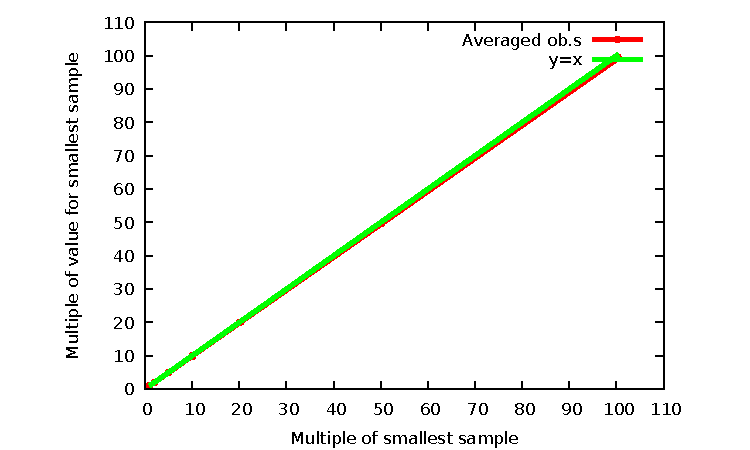
\includegraphics[width=0.505\textwidth]{\PP/SamplePlots/scaling_TREC-AP_highest_bigram_freq.pdf}}   
   \subfloat[][\IndriWT]{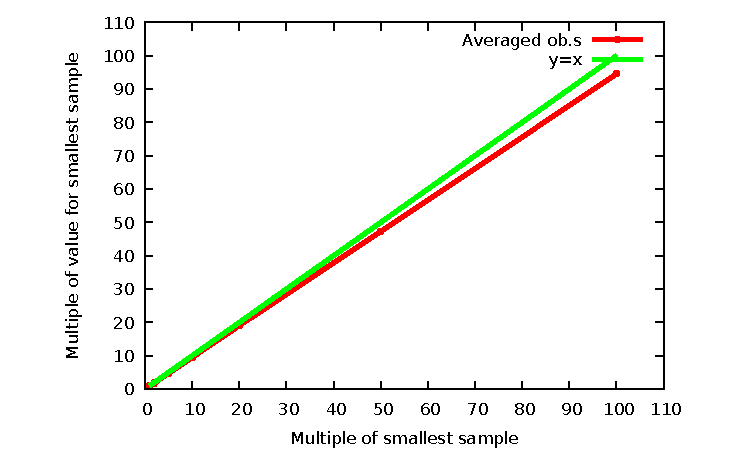
\includegraphics[width=0.505\textwidth]{\PP/SamplePlots/scaling_Indri-WT10g_highest_bigram_freq.pdf}}   

\caption{Variation of highest bigram frequency with
  corpus size for two corpora.  Note that this is a linear plot.
  \label{scalingup_bigrams_HBF}}
\end{figure}


\begin{figure}[p]
\centering
   \subfloat[][\TRECAP]{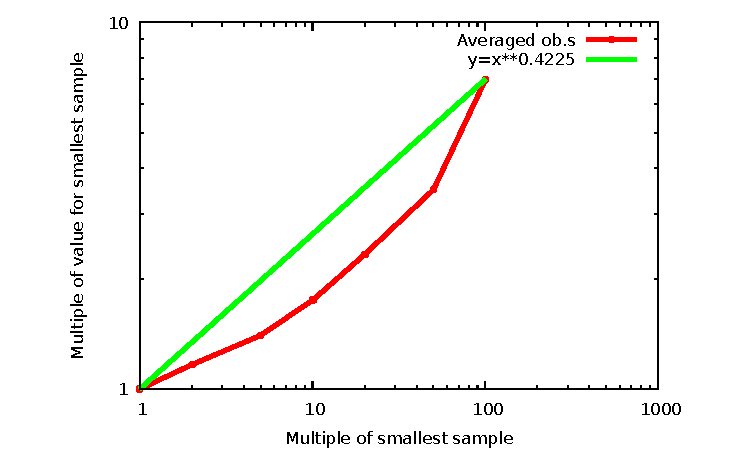
\includegraphics[width=0.505\textwidth]{\PP/SamplePlots/scaling_TREC-AP_significant_bigrams.pdf}}
   \subfloat[][\IndriWT]{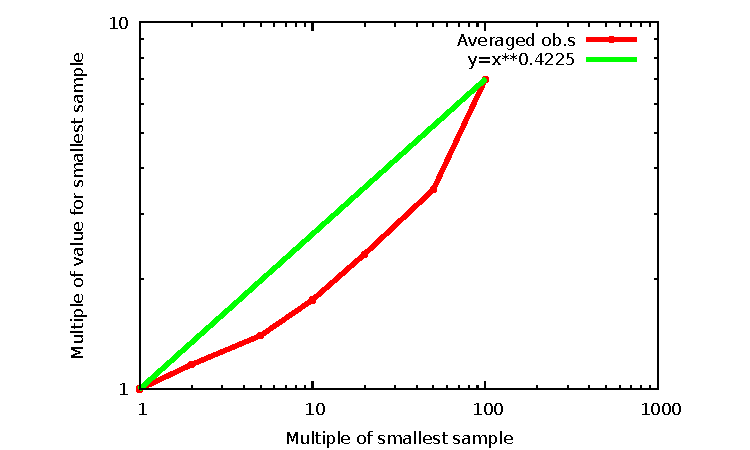
\includegraphics[width=0.505\textwidth]{\PP/SamplePlots/scaling_Indri-WT10g_significant_bigrams.pdf}}
   
\caption{Variation of number of significant bigrams with
  corpus size for two corpora.
  \label{scalingup_bigrams_NSB}}
\end{figure}


\begin{figure}[p]
\centering
   \subfloat[][\TRECAP]{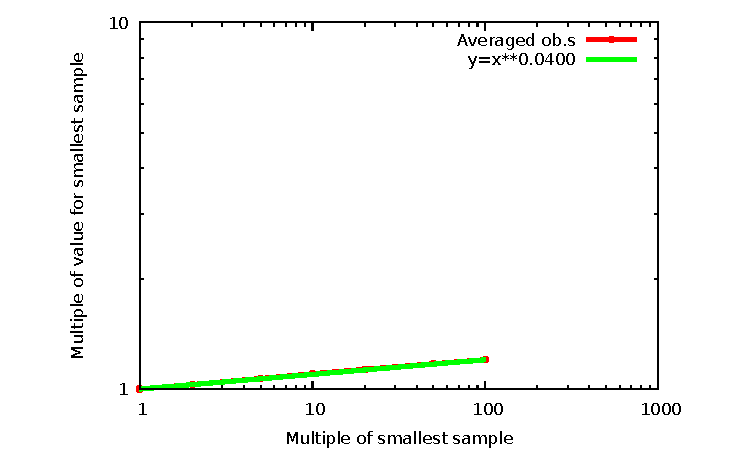
\includegraphics[width=0.505\textwidth]{\PP/SamplePlots/scaling_TREC-AP_bigram_alpha.pdf}}
   \subfloat[][\IndriWT]{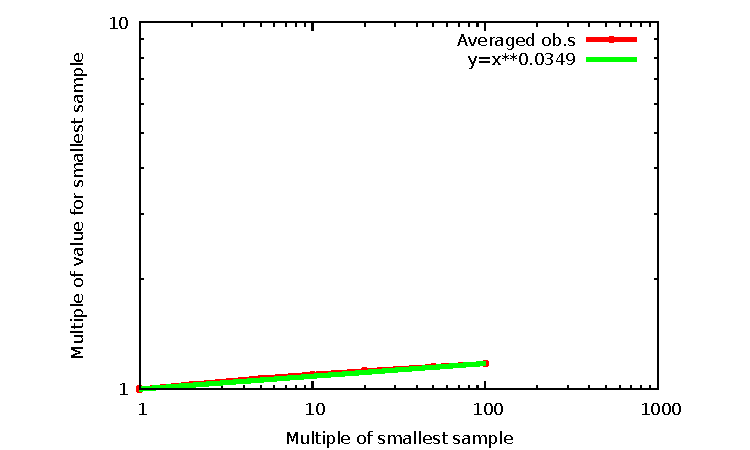
\includegraphics[width=0.505\textwidth]{\PP/SamplePlots/scaling_Indri-WT10g_bigram_alpha.pdf}}
   
\caption{Variation of exponent $\alpha$ with
  corpus size for two corpora.
  \label{scalingup_bigrams_BA}}
\end{figure}



\section{Effects of corpus growth on term dependency}

The discussion in the previous section and Figure~\ref{1-100} relate
to growth modeling with an assumption of word independence.  In this
section we start to look at how word dependence changes with increase
in corpus size.

Since we have modeled only $n$-gram associations in corpus emulations,
we start with that here.  Figure~\ref{scalingup_bigrams_HBF} suggests that 
the frequency of bigrams existing in a sample corpus grows linearly
with sample size. \todo{Can we confirm this in the shape of the
  distributions for different sample sizes?} The plots for the other
bigram parameters (Figures \ref{scalingup_bigrams_NSB} and
\ref{scalingup_bigrams_BA})
suggest a power law relationship.

The definition of ``significant bigram'' has been explained in the
section on emulation.


\chapter{Generation of compatible queries}    %%%%%%%%%%%%% Chap. 7 %%%%%%%%%%%%%
\label{QGen}

In order to study query processing efficiency and effectiveness using
a simulated text corpus, it is necessary to obtain a set of compatible
queries and judgments.  The text generation methods presented in this
paper and implemented in SynthaCorpus make no pretence of being able
to generate meaningful natural language.  Consequently it is out of
the question that ad hoc queries along the lines of those in the
TREC\footnote{\url{http://trec.nist.gov}} ad hoc task, could be
devised or judged.

In this chapter we present two alternative methods for generating
queries.  The first is due to Azzopardi \etal. It avoids the need for
human judgments by generating known-item queries appropriate to the
corpus. The second method simulates a real stream of queries and may
be used to generate realistic loads on a query processing system for
efficiency experimentation.  It cannot be used for studying
effectiveness because human judges would not be able to judge the
relevance of randomly generated documents to randomly generated queries.

\section{Azzopardi \etal~method for known-item queries}

Known-item queries allow for effectiveness evaluation in the absence
of human judgments.  Azzopardi and collaborators
\cite{AzzopardideRijke2006, AzzopardideRijkeBalog2007} have
proposed methods for automatic generation of this type of query for
real text corpora.  In essence the methods involve randomly selecting
a target document and then randomly generating a query which might be
used to retrieve it.  One of the conclusions of
\cite{AzzopardideRijkeBalog2007}
is that achieving good retrieval performance depends upon selecting suitable
targets, since humans would be much more likely to select certain
documents for re-retrieval than others.  They biased target selection
toward high-PageRank documents.

SynthaCorpus includes a query generator which implements a variant of
the method given in Equation 4 of \cite{AzzopardideRijkeBalog2007}.
Given that corpora generated by our methods
have no link structure or click information, it is not possible to
implement the Azzopardi form of target selection.  The algorithm for
generating one compatible query is shown in Algorithm \ref{algo:qgen}.

\begin{algorithm}[H]
  \begin{algorithmic}[1]
    \State \parbox[t]{.9\linewidth}{Randomly pick a target document,\
      making replacement selections if the target(s) are unsuitable.}
    \State \parbox[t]{.9\linewidth}{Randomly pick a query length $L$from\
      a distribution of query lengths.}
    \State Set the query $Q$ to empty.
    \For {$w=1$ to $L$} 
       \State \parbox[t]{.9\linewidth}{Randomly pick a word $W$ from the document, according to the \
       probabilities given by Azzopardi's Equation 4, and making a \
       replacement selection if the word has already been selected \
       in $Q$.}
       \State \parbox[t]{.9\linewidth}{Append $W$ to $Q$.}
       \EndFor
       \State \parbox[t]{.9\linewidth}{Emit $Q$.}    
  \end{algorithmic}            
  \captionof{algorithm}{The algorithim implemented in SynthaCorpus for
  generating a known-item query.  A candidate target document is
  considered unsuitable if the number of distinct words it contains is
  below a threshold $T$.  By default $T=5$.}\label{algo:qgen}
\end{algorithm}

 
\section{Modeling query streams}
Simulating the performance of query processing algorithms such as
caching requires the use of realistic query arrival sequences.  The
known-item methods in the previous section do not achieve this.
Furthermore,
generating queries from the word distribution of the target
corpus, leads to a different relationship between the word frequency
distributions of the query set and the document set.

\begin{figure}[p]
\centering
   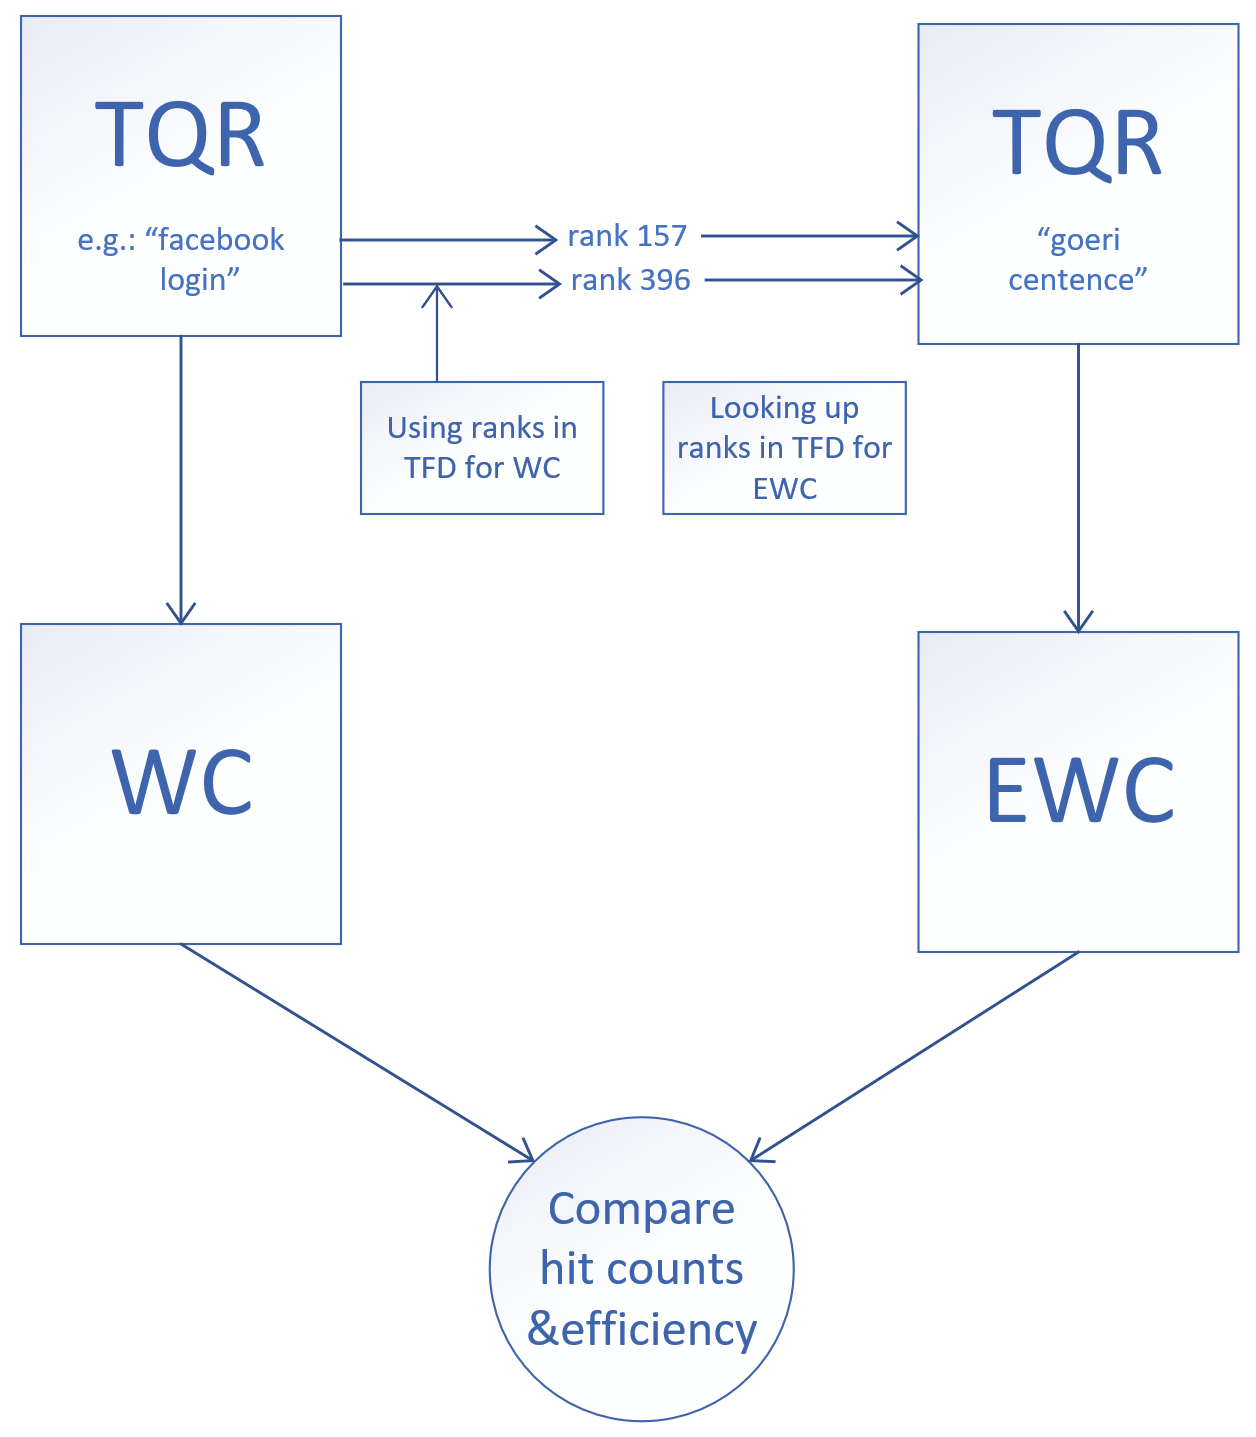
\includegraphics[width=\textwidth]{\PP/queryMappingTQRtoTQE.png}   

\caption{Queries from the real query stream TQR are converted word by
  word into queries in an emulated query stream TQE. A word from a query
  in TQR is first mapped to its rank $r$ within the word frequency distribution
  in the real web corpus WC, then the word at rank $r$ in the emulated
  corpus EWC is emitted.  The timings and hit counts when running TQR
  against WC are then compared with those for running TQE against EWC.
  If EWC very accurately mimics WC, then the two sets of observations
  should match each other closely.
  \label{emulatedWebStream}}
\end{figure}

An alternative approach is illustrated in Figure
\ref{emulatedWebStream}. The figure caption explains how the method
works.  Let us see how the proposed method can achieve accurate
emulation.

\begin{description}
\item[Word probabilities in the query stream.] In the illustration
the word ``facebook'' in the real query
stream maps to the word ``goeri'' in the emulated query stream.  Because the
same mapping is used consistently, the frequency of goeri in TQE will
inevitably be the same as the frequency of facebook in TQR.
\item[Word probabilities in the corpus.] The probability of
  occurrence of the word facebook in the real corpus WC may be very
  different to its probability of occurrence in a query stream.  This
  difference is preserved in the emulated query stream through the mapping
  via ranks, provided that the word frequency distribution is
  accurately emulated in EWC.
  \item[Word dependence] Hit counts and query latency will be affected
    by co-occurrences between the words comprising a query.  If word
    dependence is not emulated well in EWC, then we would expect there
    to be significant differences between the running of TQR against
    WC, and TQE against EWC.  Fortunately, in the Synthacorpus approach, word
    dependency modeling is based on word ranks. If facebook and login
    have a significant probability $p$ of co-occurring in WC, then
    goeri and centence should cooccur with the same probability in
    EWC.
\end{description}



We evaluate the accuracy of this form of simulation in Section \ref{webStreamSimEval}.

This approach may give us a realistic query stream, with realistic hit rates into the
target corpus.  It can't be used for ranking or effectiveness
experiments (no relevance judgments) but it can be used in efficiency
experiments, such as comparisons of different caching strategies.

\subsection{Distributing an emulated query stream}
Let us suppose that researcher Alice in industry proposes a new algorithm
for efficient processing of web queries.  She validates the algorithm by
running a private query stream \script{Q} against a private corpus
\script{C}.  In order to get her paper published she creates an
emulated version of \script{C} (i.e. \script{E}) and runs an emulated
version of \script{Q} acgainst \script{E}.  In order to allow a fellow
researcher Bob at another institution (possibly a rival company) to
reproduce her results she
sends Bob the parameters used to generate \script{E} and includes the
random seed so that B's version of \script{E} will be identical to
hers.  The next question is how to allow Bob to share the same query
stream.  Distributing the emulated query stream in text form would work, as long as
Bob's version of \script{E} is identical to Alice's.  Alternatively,
the words in the original query log could be represented as rank-based
term-ids, to reduce the dependence on exact replication of \script{E}.

A downside is that the query stream probably substantially increases the
size of the information which Alice must pass on to Bob.  We could, of course,
model the stream as though it were a document collection using the
methods discussed in preceeding chapters -- query length model, word
frequency model, term dependence model, and term representation model.
Unfortunately, the effectiveness of a caching model relies on the
arrival sequence of the queries -- there are dependences across
``document'' (i.e. query) boundaries.  When a searcher reformulates a query,
temporally close queries are likely to re-use the same or related
words; The distribution of query words at any point in time will
depend upon the group of users who are active at that time.  If we
distribute a compact parameterized model of the query stream along the
lines so far discussed, we will
lose important aspects of the stream.  Bob may not be able to
reproduce Alice's results.  If Alice used the same compact model
as Bob, their results would agree but they might not agree with
Alice's orgiginal results obtained on the real data.


On the other hand, despite its flaws, the compact model might be
better able to preserve privacy.  


\subsection{Privacy considerations}
The non-compact form of the emulated query stream can be seen as an encrypted form
of the original, where the encryption algorithm is a fixed
word-for-word substitution cypher.  An adversary Eve may be able to
use external information such as expected word frequencies, and
likely n-grams to decode at least some of the queries.   Eve
may be aided by information about the sequence of queries.

To a non-expert eye it seems unlikely that this decoding process would
succeed in decrypting many of the infrequently occurring
words, such as people's names and credit card numbers.   The
encryption might be sufficient to avoid the problems exposed in the
AOL query log distribution, which were in any case dramatically
magnified by the presence of session identifiers.

The compact model provides better protection against attack because
it adds randomness to the word mappings and because it removes all
vestiges of the original query sequence.

If the query stream contains highly sensitive information such as
searches by a chemical company against a patent index, Eve would likely be
highly motivated.  In this circumstance it would be wise to use the
compact model or to avoid
sharing even emulated data.



\chapter{Approaches to evaluating synthetic test collections}   %%%%%%%%%%%%% Chap. 8 %%%%%%%%%%%%%
\label{chap:SynEval}

Previous chapters have presented alternative approaches to each of the
different modeling dimensions which vary in their ability to
faithfully model a corpus; Some of the approaches can be more
or less faithful depending upon settings such as the number of segments
in a piecewise linear model. There is clearly a need to devise suitable evaluation methodologies
for comparing different approaches and for measuring how faithfully an emulated
collection matches the corresponding real one.


\section{Task based evaluation}
The most practically
important forms of evaluation are those derived from the task for
which the emulated collection was created:
\begin{itemize}
  \item How well do observations on that task, (e.g. indexing speed, query
    response latency, ranking accuracy, learning to rank etc.) predict those obtained
    on the corresponding real collection?
\end{itemize}

When working with a private corpus, the ability to accurately predict real
behaviour on the dimensions we care about is all we care about.  We
need to be able to do this in the presence of constraints on what we
are allowed to extract from the private data.

Chapter \ref{Indri-experiments} presents some illustrative evaluations along
these lines, using an open-source IR system and the words and document
boundaries from a well-known test corpus.


\section{Non-task based evaluation}
Using task-based evaluation allows us to measure the end-to-end
performance of a simulation but we may need finer-grained evaluations
to understand why observations from a simulated collection fail to
predict behaviour on a real system.  For example, if we observe that
indexing of a real corpus \script{C} is substantially faster or slower than
indexing of an emulated version \script{E}, we may want to compare
vocabulary sizes, word-frequency distributions, document length
distributions, word-length distributions, etc. of \script{E} and
\script{C}.  Finding a substantial difference in say word frequency
distributions would suggest changing that model.

Some of the modeling parameters are simple numeric quantities and can
be easily compared.  There are are a number of possible ways to compare two
distributions:

\subsection{Comparing distributions: visual method}

A method which has been used without discussion in earlier chapters
is that of plotting two distributions on a single set of axes, usually
log-log, in order to allow visual comparison.  Visual comparison has the 
advantage that it gives a very clear indication (see Figure \ref{Blah} for example) when
the  distributions for \script{E} and
\script{C} vary substantially.  It can also clearly indicate
how the two distributions differ.  For example, the plots have
different shapes, or the slopes of the lines differ, or the domains of
the plots have different sizes.

It should not be forgotten that a
corpus generated by random sampling is only one of an infinite number
of possible outcomes.  Distributional plots for different corpora
generated with the same generation parameters are likely to vary. 

As long as caution is used 
and the distributions are plotted appropriately visual comparison can
be a very useful method, arguably the most useful.

On the other hand visual comparison has the disadvantage that it
doesn't result in a single-dimensional measure of difference.  This is
a limitation when we want to compare two different emulation methods
-- Which of the two emulated distributions is closest to the real one?


\subsection{Comparing distributions: Kolmogorov Smirnov}
A variant of the Kolmogorov-Smirnov (K-S) test is able test the null
hypothesis that two discrete cumulative probability distributions represent
samples drawn from the same population.  Informally, the K-S statistic
measures the greatest vertical divergence between the two cumulative
distributions.

We could, for example, use a K-S test with suitably chosen confidence
criterion to accept or reject the null
hypothesis that the word probability distributions for \script{E} and
\script{C} have been drawn from the same population.



\subsection{Comparing distributions: Kullback-Leibler divergence}

Kullback-Leibler (KL) divergence can give us an information theoretic
measure of the extent to which a discrete probability distribution (e.g. of word
probabilities) from \script{E} diverges from that of \script{C}.  If a
single number measure of difference between two distributions is
required, then the KL divergence $D_{KL}$of \script{E} from \script{C}
seems like a good choice.  

\[ D_{KL}(\mathscr{E}||\mathscr{C}) = \sum_i \mathscr{E})_i\frac{\mathscr{E}_i}{\mathscr{C}_i} \]

Usually, in language modeling work, $\mathscr{E}_i$ and $\mathscr{C}_i$
relate to the same word. That is not generally the case in corpus
synthesis, where the probabilities being compared are those of
different words which happen to appear at the same rank.  This doesn't
seem to be an important issue.

A more important issue is that, since \script{E} is generated by a random
process, the measured KL divergence applies
only to that specific generated instance.  To correctly measure the
fidelity of an emulation method, one would have to generate a large
number of \script{E}s and average their KL divergence scores.

Another issue is that the vocabularies of \script{E} and \script{C}
may differ in size.  If the vocabulary size of \script{C} is smaller,
then for some words, $\mathscr{C}_i = 0$ but $\mathscr{E}_i \ne 0$,
violating an assumption of the measure.  This is simply solved by
smoothing, i.e. setting zero values to a small non-zero value.

In our work, KL divergences can be measured for probability distributions for
words frequencies, $n$-gram frequencies, co-occurrence frequencies,
self-cooccurrence frequencies, document lengths, and word lengths.
Averaged KL divergences could be used to compare the fidelity of one
emulation method with that of another.




\chapter{Emulation experiments assuming word independence}   %%%%%%%%%%%%% Chap. 9 %%%%%%%%%%%%%
\label{EmExpts}

\begin{figure}[p]
\centering
\subfloat[][\TRECAP]{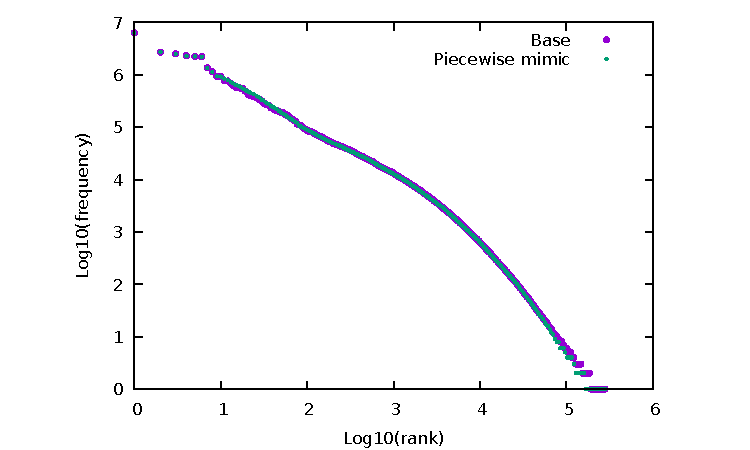
\includegraphics[width=0.505\textwidth]{\PP/Piecewise/markov-5e_dlhisto_ind/TREC-AP_base_v_mimic_unigrams.pdf}}
\subfloat[][\TopQ]{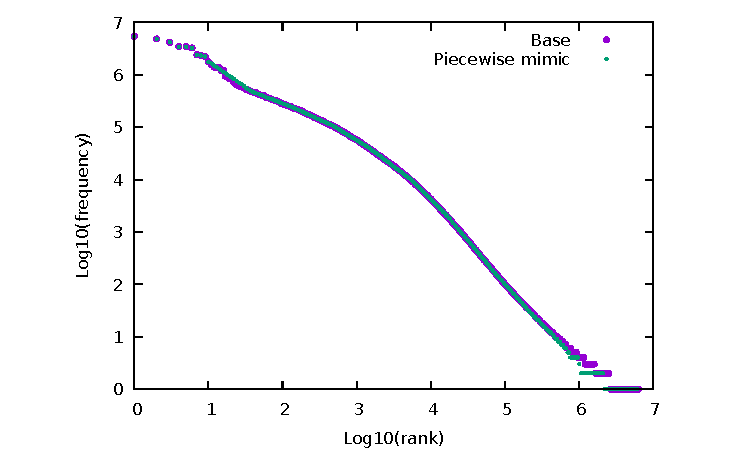
\includegraphics[width=0.505\textwidth]{\PP/Piecewise/markov-5e_dlhisto_ind/Top100M_base_v_mimic_unigrams.pdf}}

\subfloat[][\classificationPaper]{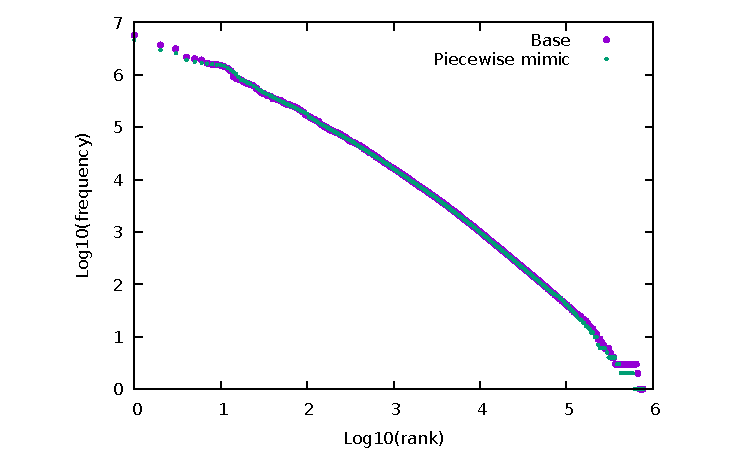
\includegraphics[width=0.505\textwidth]{\PP/Piecewise/markov-5e_dlhisto_ind/classificationPaper_base_v_mimic_unigrams.pdf}}
\subfloat[][\Wikipedia]{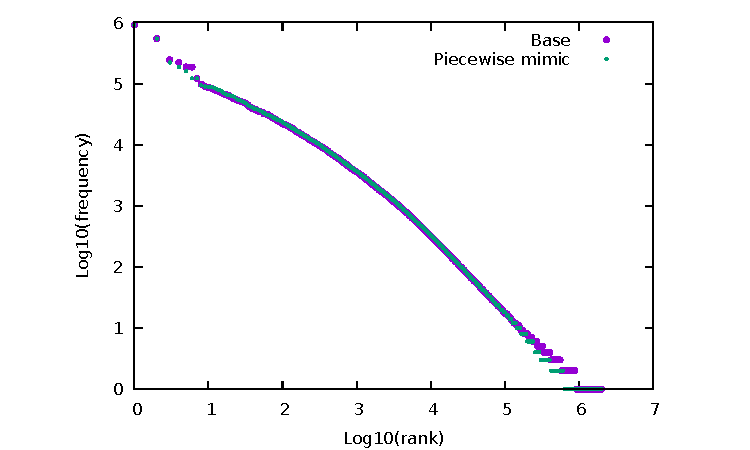
\includegraphics[width=0.505\textwidth]{\PP/Piecewise/markov-5e_dlhisto_ind/Wikipedia_base_v_mimic_unigrams.pdf}}

\subfloat[][\AcademicID]{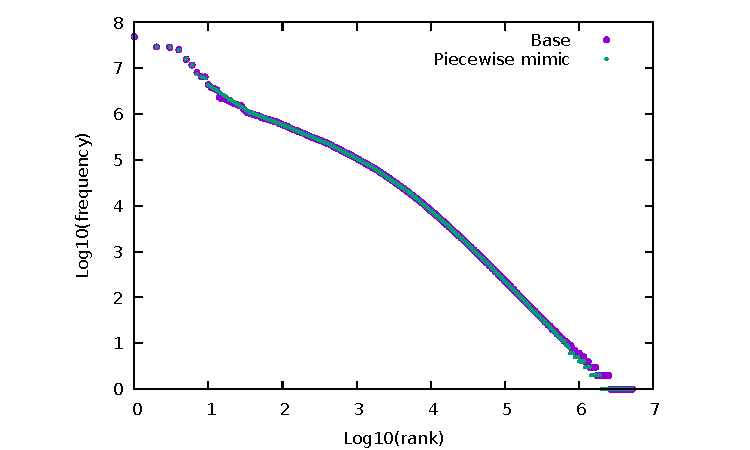
\includegraphics[width=0.505\textwidth]{\PP/Piecewise/markov-5e_dlhisto_ind/AcademicID_base_v_mimic_unigrams.pdf}}
\subfloat[][\IndriWT]{\includegraphics[width=0.505\textwidth]{\PP/Piecewise/markov-5e_dlhisto_ind/INdri-WT10g_base_v_mimic_unigrams.pdf}}

\caption{Base-versus-emulated word frequency distributions in log-log space for a
  selection of the corpora.  Word frequency modeling was done using
  the three-part, piecewise model with $h=10, s=10$.
\label{fig:independentUnigrams}}
\end{figure}

\begin{figure}[p]
\centering
\subfloat[][\TRECAP]{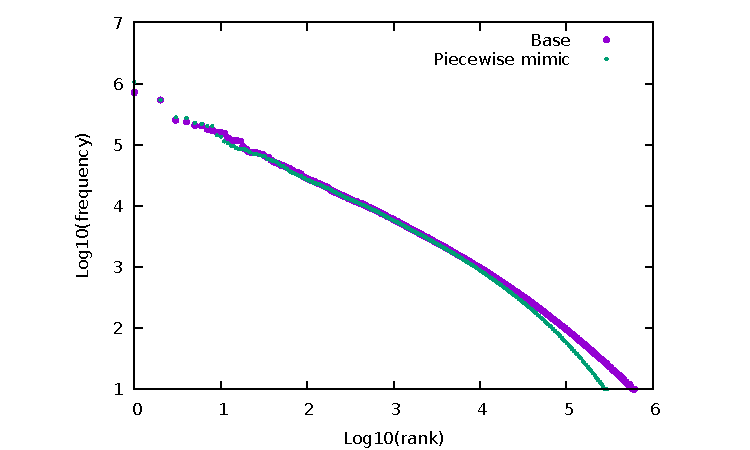
\includegraphics[width=0.505\textwidth]{\PP/Piecewise/markov-5e_dlhisto_ind/TREC-AP_base_v_mimic_bigrams.pdf}}
\subfloat[][\TopQ]{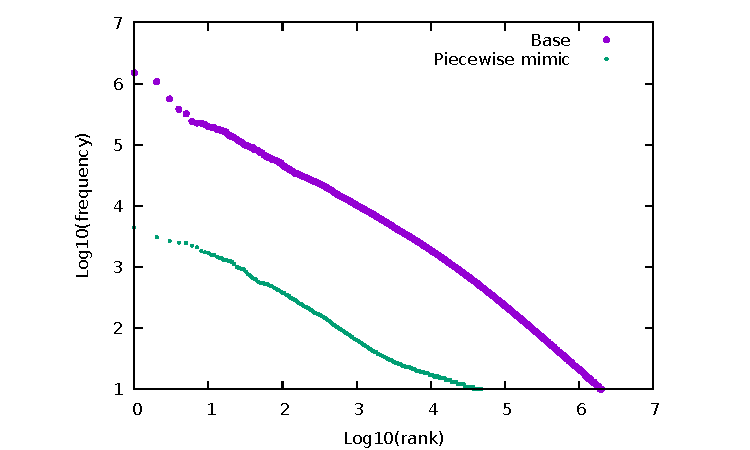
\includegraphics[width=0.505\textwidth]{\PP/Piecewise/markov-5e_dlhisto_ind/Top100M_base_v_mimic_bigrams.pdf}}

\subfloat[][\classificationPaper]{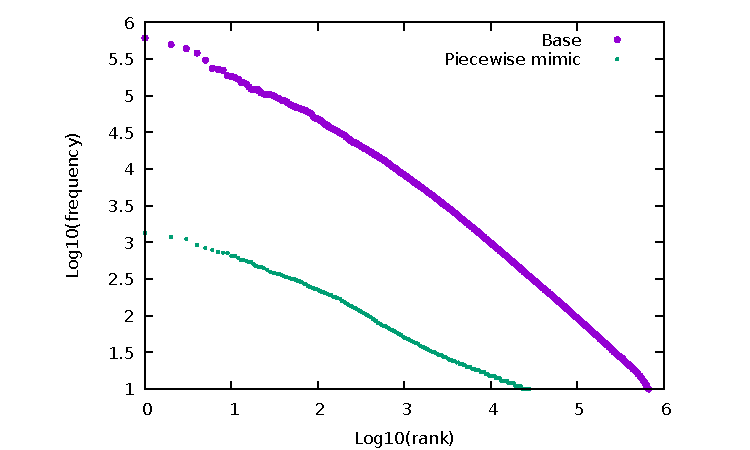
\includegraphics[width=0.505\textwidth]{\PP/Piecewise/markov-5e_dlhisto_ind/classificationPaper_base_v_mimic_bigrams.pdf}}
\subfloat[][\Wikipedia]{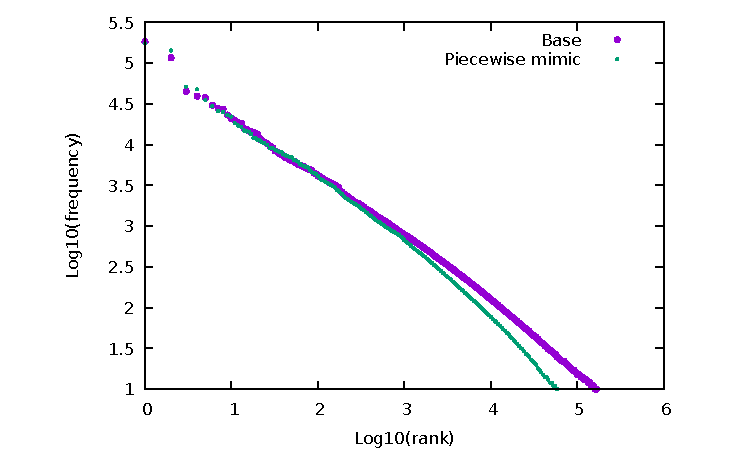
\includegraphics[width=0.505\textwidth]{\PP/Piecewise/markov-5e_dlhisto_ind/Wikipedia_base_v_mimic_bigrams.pdf}}

\subfloat[][\AcademicID]{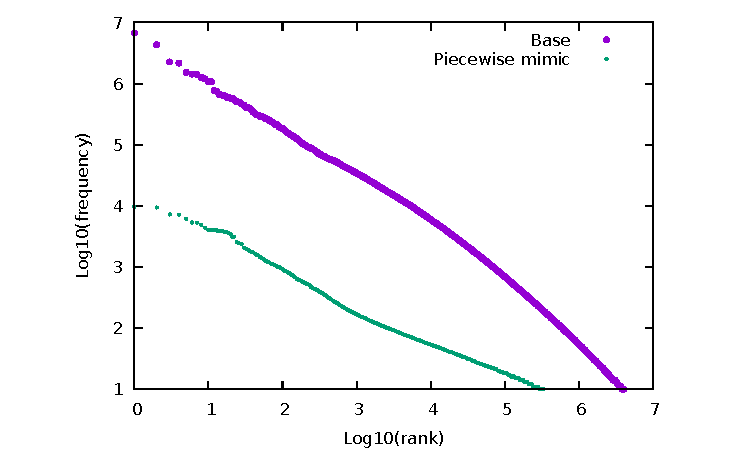
\includegraphics[width=0.505\textwidth]{\PP/Piecewise/markov-5e_dlhisto_ind/AcademicID_base_v_mimic_bigrams.pdf}}
\subfloat[][\IndriWT]{\includegraphics[width=0.505\textwidth]{\PP/Piecewise/markov-5e_dlhisto_ind/INdri-WT10g_base_v_mimic_bigrams.pdf}}

\caption{Base-versus-emulated bigram frequency distributions in log-log space for a
  selection of the corpora.  Word frequency modeling was done using
  the three-part, piecewise model with $h=10, s=10$.
\label{fig:independentBigrams}}
\end{figure}



For each of the corpora we used the SynthaCorpus
\texttt{emulateARealCorpus.pl} script to produce a synthetic emulated
version. In a series of figures we present
base-versus-emulated comparison results for various modeling
dimensions.

Figure~\ref{fig:independentUnigrams} presents comparisons of word
frequency distributions for the case where emulation uses a
sophisticated model.  As may be seen, modeling is very accurate.
In contrast, Figure~\ref{fig:independentBigrams} compares the
distribution of significant bigrams when the emulation assumes
word independence.  Modeling of bigram frequencies is very poor - the
number of significant bigrams found in the emulated corpus is an order of magnitude less, and
the frequency of the most frequent bigram is almost two orders of
magnitude less.   In the next chapter, we will see that this gap can
be effectively closed if we use $n$-gram modeling.

\todo{We need to add comparisons of word length distributions.
  Annoyingly these don't currently seem to be produced.}




%For additional confirmation, we produced
%cumulative probability plots for real and emulated corpora and carried out
%Kolmogorov-Smirnov testing\footnote{See
%e.g.~\url{https://en.wikipedia.org/wiki/Kolmogorov\%E2\%80\%93Smirnov_test}.}
%These are shown in Figure~\ref{KS}.  

%\todo{Do we need to say: We follow \cite{clausetShaliziNewman2009powerLawDistributions} and use
%the Kolmogorov-Smirnov
%test~\cite{pressTeukolskyVetterlingFlannery1992numericalRecipes}.
%}

\chapter{Emulation with word dependence modeling}    %%%%%%%%%%%%% Chap. 10 %%%%%%%%%%%%%
\label{chap:dependenceExpts}


\begin{figure*}[p]
  \centering

  % The file we want will be in
  % GIT/SynthaCorpus/Experiments/Emulation/Piecewise/markov-5e_dlhisto_ind/TREC-AP_base_v_mimic_bigrams.pdf
%\subfloat[][Independence]{\includegraphics[width=0.505\textwidth]{\PP/PiecewisePlots/TREC-AP_markov-5e_dlhisto_ind/base_v_mimic_bigrams.pdf}}
  % The file we want will be in
  % GIT/SynthaCorpus/Experiments/Emulation/Piecewise/markov-5e_dlhisto_ngrams2/TREC-AP_base_v_mimic_bigrams.pdf
%\subfloat[][Modeling 2-grams]{\includegraphics[width=0.505\textwidth]{\PP/PiecewisePlots/TREC-AP_markov-5e_dlhisto_ngrams2/base_v_mimic_bigrams.pdf}}

\caption{Bigram frequency distributions in log-log space for the
  \TRECAP~corpus. Note that in this figures and the following series of
  figures, for both base and emulated corpora, only bigrams which occur more frequently than
  would be expected in a random scatter model are considered.  Each graph plots bigram frequencies observed
  in the relevant corpus (base or emulated) and selected using identical decision
  criteria.   
\label{fitAP}}
\end{figure*}

\begin{figure*}[p]
\centering
%\subfloat[][Independence]{\includegraphics[width=0.505\textwidth]{\PP/PiecewisePlots/Indri-WT10g_markov-5e_dlhisto_ind/base_v_mimic_bigrams.pdf}}
%\subfloat[][Modeling 2-grams]{\includegraphics[width=0.505\textwidth]{\PP/PiecewisePlots/Indri-WT10g_markov-5e_dlhisto_ngrams/base_v_mimic_bigrams.pdf}}

\caption{Bigram frequency distributions in log-log space for the
  \IndriWT~corpus.
\label{fitWT}}
\end{figure*}

\begin{figure*}[p]
\centering
%\subfloat[][Independence]{\includegraphics[width=0.505\textwidth]{\PP/PiecewisePlots/clueWeb12BodiesLarge_markov-5e_dlhisto_ind/base_v_mimic_bigrams.pdf}}
%\subfloat[][Modeling 2-grams]{\includegraphics[width=0.505\textwidth]{\PP/PiecewisePlots/clueWeb12BodiesLarge_markov-5e_dlhisto_ngrams/base_v_mimic_bigrams.pdf}}

\caption{Bigram frequency distributions in log-log space for the
  \clueWebBodiesLarge~corpus.
\label{fitCWB}}
\end{figure*}


\begin{figure*}[p]
\centering
%\subfloat[][Independence]{\includegraphics[width=0.505\textwidth]{\PP/PiecewisePlots/AcademicID_markov-5e_dlhisto_ind/base_v_mimic_bigrams.pdf}}
%\subfloat[][Modeling 2-grams]{\includegraphics[width=0.505\textwidth]{\PP/PiecewisePlots/AcademicID_markov-5e_dlhisto_ngrams2/base_v_mimic_bigrams.pdf}}

\caption{Bigram frequency distributions in log-log space for the
  \AcademicID~corpus.
\label{fitAC}}
\end{figure*}


\begin{figure*}[p]
\centering
%\subfloat[][Independence]{\includegraphics[width=0.505\textwidth]{\PPlap/PiecewisePlots/Wikipedia_markov-5e_dlhisto_ind/base_v_mimic_bigrams.pdf}}
%\subfloat[][Modeling 2-grams]{\includegraphics[width=0.505\textwidth]{\PPlap/PiecewisePlots/Wikipedia_markov-5e_dlhisto_ngrams/base_v_mimic_bigrams.pdf}}

\caption{Bigram frequency distributions in log-log space for a
  \Wikipedia~corpus. 
\label{fitWK}}
\end{figure*}


\begin{figure*}[p]
\centering
%\subfloat[][Independence]{\includegraphics[width=0.505\textwidth]{\PPlap/PiecewisePlots/classificationPaper_markov-5e_dlhisto_ind/base_v_mimic_bigrams.pdf}}
%\subfloat[][Modeling 2-grams]{\includegraphics[width=0.505\textwidth]{\PPlap/PiecewisePlots/classificationPaper_markov-5e_dlhisto_ngrams/base_v_mimic_bigrams.pdf}}

\caption{Bigram frequency distributions in log-log space for a
  \classificationPaper~corpus. 
\label{fitCP}}
\end{figure*}


\begin{figure*}[p]
\centering
%\subfloat[][Independence]{\includegraphics[width=0.505\textwidth]{\PPlap/PiecewisePlots/Top100M_markov-5e_dlhisto_ind/base_v_mimic_bigrams.pdf}}
%\subfloat[][Modeling 2-grams]{\includegraphics[width=0.505\textwidth]{\PPlap/PiecewisePlots/Top100M_markov-5e_dlhisto_ngrams/base_v_mimic_bigrams.pdf}}

\caption{Bigram probability distributions in log-log space for a
  \TopQ~corpus. 
\label{fitTM}}
\end{figure*}




%%%%%%%%%%%%%%%%%%%%%%%%%%%%%%%%%%%%%%%%%%%%%%%%%%%%%%%%%%%%%%%%%%%%%%%%%%%%%%%%%%%%%%%%%%%%%%%%%%%%%%%%%%%%%%%%%%%%%%


\begin{figure*}[p]
\centering
%\subfloat[][Modeling 2-grams]{\includegraphics[width=0.34\textwidth]{\PP/PiecewisePlots/TREC-AP_markov-5e_dlhisto_ngrams2/base_v_mimic_bigrams.pdf}}
%\subfloat[][Modeling 2,3-grams]{\includegraphics[width=0.34\textwidth]{\PP/PiecewisePlots/TREC-AP_markov-5e_dlhisto_ngrams3/base_v_mimic_bigrams.pdf}}
%\subfloat[][Modeling 2,3,45-grams]{\includegraphics[width=0.34\textwidth]{\PP/PiecewisePlots/TREC-AP_markov-5e_dlhisto_ngrams5/base_v_mimic_bigrams.pdf}}

\caption{Bigram frequency distributions in log-log space.  Exploring
  the effect of increasing the degree of $n$-gram modeling for
  the\TRECAP~corpus. Moving from (a) to (c) shows the effect of including
  progressively higher order $n$-grams in the emulation process.
\label{fitAP2}}
\end{figure*}


\begin{figure*}[p]
\centering
%\subfloat[][Modeling 2-grams]{\includegraphics[width=0.34\textwidth]{\PP/PiecewisePlots/AcademicID_markov-5e_dlhisto_ngrams2/base_v_mimic_bigrams.pdf}}
%\subfloat[][Modeling 2,3-grams]{\includegraphics[width=0.34\textwidth]{\PP/PiecewisePlots/AcademicID_markov-5e_dlhisto_ngrams3/base_v_mimic_bigrams.pdf}}
%\subfloat[][Modeling 2,3,45-grams]{\includegraphics[width=0.34\textwidth]{\PP/PiecewisePlots/AcademicID_markov-5e_dlhisto_ngrams5/base_v_mimic_bigrams.pdf}}

\caption{Ditto for
  the\AcademicID~corpus. 
\label{fitAc2}}
\end{figure*}


\chapter{Experiments with word representation methods}   %%%%%%%%%%%%% Chap. 11 %%%%%%%%%%%%%
\label{chap:wordRepExpts}
We are concerned with three criteria: the quality of the terms
generated by each method, and the memory and runtime cost of the method
itself.  All our validation experiments involve taking the vocabulary
of a real (seed) corpus, generating a synthetic vocabulary of the same size,
and comparing the properties of the two.  We report results for
Clueweb12~\cite{clueweb12}; space doesn't permit presentation of
broadly similar results for the TREC Associated Press documents 
and a collection of 
academic paper titles.

\paragraph*{Term quality}

For most experimental purposes, we want synthetic terms to ``look
like'' real terms from (e.g.) English web pages. To evaluate our
methods on these grounds we use three criteria. First, \textbf{term
  lengths} should be distributed similarly to the seed corpus. Second
and third, \textbf{character distribution} and \textbf{bigram
  distribution} should match. In each case we measure the
Jensen-Shannon divergence~\cite{Lin1991} between the seed and synthetic
distributions: this measures the difference between two multinomial
distributions and ranges from~0 (the two distributions are identical)
to 1~(they are completely dissimilar).\footnote{Note that we used
  logarithms with base 2.} 

We must also consider the way generated terms behave in typical
components of an IR system.  A wide range of vocabulary accumulation
structures are reviewed by \citet{HeinzZW2002}.  Comparing
the suitability of synthetically generated terms against all of these
methods is beyond the scope of the present work, but as a sanity
check, we consider the rate of hash collisions---that is, how many
terms share hashes? This clearly depends crucially on the choice of
hash function and table size, but serves to illustrate the sorts of
downstream processing needed in a real IR system. The goal is not, of
course, to minimise collisions; rather it is to generate terms which
behave similarly to those in the seed corpus.  We used the FNV-1a %(op. cit.)
hashing method and set the table
size to the smallest power of two which was at least 20\% larger than
the vocabulary size.

Finally, we report the number of generated terms which were also seen
in our seed corpus: that is, the number of times each method
coincidentally generated a ``real'' word.

\paragraph*{Runtime requirements}

Synthetic corpora are likely to be used in performance and scalability
testing. If synthetic term generation uses a lot of memory or
computation, then it may interfere with the test; on the other hand,
if it can be done fast and with minimal memory then it would be
possible to embed the generator into the indexer or other component
being studied.

We report memory use and CPU time, based on a single indicative run,
but note that optimisation has not been a focus and these timings
should be interpreted as indicative only. Tests were run
single-threaded on a server using Intel Xeon(R) CPU E5-2643 CPUs
running at 3.30GHz,and with 64GB of RAM and RAID storage.  Reading 
the seed vocabulary and building all the transition matrices and other 
structures took a little over 3 minutes elapsed.

We note that the Base26 and Base26-sparsity
methods do not rely on shared read-write structures and could easily be
multi-threaded.  However, methods (all the others) which can potentially generate the
same term at different ranks, would require locking of the hashtable
used to detect and avoid this.

\paragraph*{Results}
\begin{figure*}
\centering
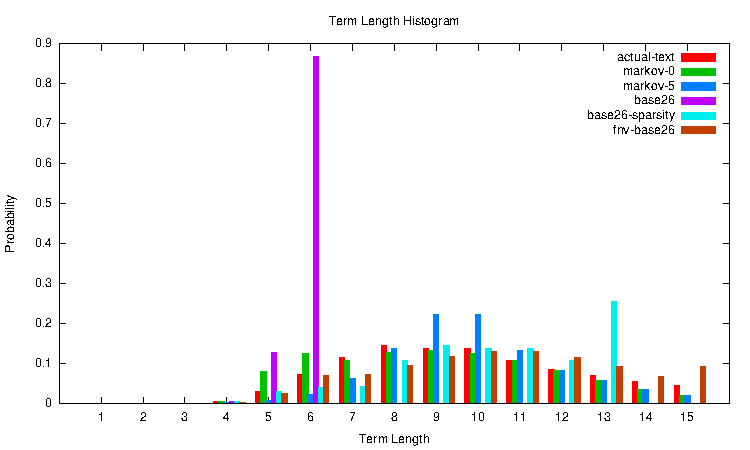
\includegraphics[width=0.7\textwidth]{images/ClueWeb12/termLengthHistogram.pdf}
\caption{Term length histogram for the ClueWeb12 corpus and various
  simulated methods. \label{plots} }
\end{figure*}


Results are summarised in Table~\ref{tab:summary}, which shows quality
scores for 89,536,745~terms generated with Clueweb12 as seed.  The
methods which use the length model (Markov-$*$ and FNV-Base26) closely
emulate
the length distribution of the seed corpus;  Base26 performs very
poorly while Base26-sparsity may be accurate enough. Perhaps
surprisingly, all methods
perform fairly well on the unigram distribution.  Unsurprisingly the
higher order Markov models perform best on the bigram distribution.
Choice of method has almost no effect on hash collision rate.  The
Base26 methods are much faster than the Markov ones, and the higher
the Markov order, the slower the method.  Much of the slow down is due
to the need to generate and test more candidates for uniqueness.  The
slowest method is more than three hundred times slower than the fastest.

\todo{Co-authors like table tab:summary. Can we generate similar
  tables for other simulation dimensions?  And include CPU/memory numbers?}

Figure \ref{plots} shows the term length distributions of the methods
-- some of the Markov methods are omitted for clarity.  The inherent deficiency
of the Base26 method shows clearly in the spike at length 6, while the
peak at length 13 for the Base26-sparsity method is believed to be due
to measures taken to avoid overflowing the 64 bit integer from
which the base 26 string is generated.


\begin{table*}[t] \tiny
\centering
\caption{ Summary characteristics of the term generation methods. $k$
  is the order of the Markov model. Lengths and character
  distributions are measured with Jensen-Shannon divergence, which
  ranges from 0 (identical) to 1 (completely dissimilar). Using 
  a FNV-1A hash reduced to 27 bits, 27.038\% of terms in the original 
  vocabulary hashed to a slot already occupied by another time. Hash 
  collisions record the result of dividing the corresponding
  percentage for each method by 27.038\%. Memory and
  runtimes are to generate 89,536,745 terms and are
  approximate.``HT'' is the size of the hashtable used to detect
  duplicates. In our implementation, HT was 2560MB.   The number of tries per word is the average number of
  candidates generated before finding one which had not been used
  before.  The time/word includes all the unsuccessful tries.}
\label{tab:summary}
\begin{tabular}{rcccccccc}
%\toprule
             & \multicolumn{3}{c}{JS divergence} & Terms      & Hash       & State  & \multicolumn{2}{c}{Time/word} \\
             & Lengths & Unigrams & Bigrams      & in seed (M)& collisions & memory & $\mu$s & Tries                \\
\cmidrule(lr){2-4}\cmidrule(lr){5-5}\cmidrule(lr){6-6}\cmidrule(lr){7-7}\cmidrule(lr){8-9}
%Clueweb12    &      &      &                     &  89.5      &            &         &      &                       \\[.5em]
Base26       & 0.7551  & 0.0852  & 0.2388    & \Z4.9      & 1.0013     & 0       & \Z0.12 & \Z1.0               \\
Base26-sparsity 
             & 0.1095  & 0.0906  & 0.2460   & \Z1.0      & 0.9998     & 16-word array & \Z0.22 & \Z1.0    \\
FNV-Base26   & 0.0192  & 0.0852 & 0.2387    & \Z0.8      & 0.9996     & HT      & \Z0.86 & \Z1.1               \\
Markov $k=0$ & 0.0200  & 0.0085  & 0.0906   & \Z4.0      & 0.9999     & HT+$\ll$1MB   & \Z3.72 & \Z5.8    \\
\hfill $k=1$ & 0.0176  & 0.0118 & 0.0558    & \Z5.9      & 1.0002     & HT+$\ll$1MB   & \Z5.81 & \Z8.6    \\
\hfill $k=2$ & 0.0182  & 0.0099 & 0.0448    & \Z6.1      & 1.0001     & HT+$<$1MB     & \Z9.14 & 12.3     \\
\hfill $k=3$ & 0.0171  & 0.0047 & 0.0230    & \Z5.9      & 0.9996     & HT+4MB    & 15.63 & 18.1               \\
\hfill $k=4$ & 0.0229  & 0.0025 & 0.0127    & \Z6.2      & 0.9997     & HT+105MB  & 24.17 & 23.3               \\
\hfill $k=5$ & 0.0422  & 0.0019 & 0.0102    & \Z5.9      & 0.9994     & HT+2846MB & 43.78 & 34.2               \\
\bottomrule
\end{tabular}
\end{table*}

\section{Discussion of term representations}

The term lists produced by the higher order Markov
methods we implemented show quite good distributions of length,
unigram frequency and bigram frequency.  Particularly with smoothing
enabled, they are capable of generating vocabularies far larger than
the one used for training. Subjectively, there is
a plausibility to many of the terms they generate: e.g.\ ``bayesiant'',
``biopestive'', ``relaxationalco''.  However, our
method cuts off the letter chains at a pre-selected length,
resulting in many unnatural word endings.  This potential problem could be
addressed by avoiding the length model and including an END symbol 
in the alphabet.  To model the dependence of term length on term rank,
we propose using multiple START symbols based on the rank buckets in
Table~\ref{length_model}.  

Unfortunately, the Markov methods require far too much memory for use
in embedded efficiency experiments.  This is because the need for
large, randomly accessed data structures causes flushing of CPU caches
and consequent serious interference with algorithms being studied.  In
other off-line generation scenarios they may be preferred.

In embedded applications the Base26-sparsity method seems the best
choice.  It requires only a small table of skip values (15 in our
case), generates better terms than base26, and is capable of
generating almost 5 million terms per second, single threaded.  However, generating a
scaled-up vocabulary would require a model of how the skip table entries
change with vocabulary size. Speed of generation can
easily be improved by multi-threading and probably by code
optimisation.  A disadvantage of the method is that terms sorted by
rank are also sorted by length, i.e. all the $n$-letter terms have
lower ranks than any of the terms with $n + 1$ letters.  A solution to
this might lie in using the length model to choose the length $L$ of a
term and then using the skip value for $L$ to compute a term
number.  An extra counter for each length and a fallback mechanism
would be needed to ensure that repeated terms were not generated but
total memory requirement would still be only around 30 numbers.

Reproducibility of experiments involving synthetic term generation is
an important desideratum.  Base26 for an
agreed alphabet is inherently reproducible and base26-sparsity
requires only the additional sharing of a small table of skip values.
Reproducible term generation by the stochastic methods is more
challenging.  It requires communication of the random seed, and the
table of parameters to the length model.  A reproducible
Markov generator would additionally require communication of the 
transition matrix.

 
\begin{figure*}
\centering
    %\subfloat[][\TRECAP]{\includegraphics[width=0.33\textwidth]{\PP/LinearPlots/TREC-AP_real_v_mimic.pdf}}
    %\subfloat[][\AcademicID]{\includegraphics[width=0.33\textwidth]{\PP/LinearPlots/AcademicID_real_v_mimic.pdf}}
    %\subfloat[][\clueWebTitles]{\includegraphics[width=0.33\textwidth]{\PP/LinearPlots/clueWeb12Titles_real_v_mimic.pdf}}

    %\subfloat[][\TRECAP]{\includegraphics[width=0.33\textwidth]{\PP/PiecewisePlotsPlots/TREC-AP_real_v_mimic.pdf}}
    %\subfloat[][\AcademicID]{\includegraphics[width=0.33\textwidth]{\PP/PiecewisePlotsPlots/AcademicID_real_v_mimic.pdf}}
    %\subfloat[][\clueWebTitles]{\includegraphics[width=0.33\textwidth]{\PP/PiecewisePlotsPlots/clueWeb12Titles_real_v_mimic.pdf}}
\caption{Term probability
  distributions of base corpora \script{C} and corresponding emulated
  corpora \script{E}.  Top row shows linear emulation ($h=10, s=1$)
  while bottom row shows piecewise linear emulation ($h=10, s=10$)
  for the same corpora. \label{emulation} }
\end{figure*}



\chapter{Scaling-up experiments}  %%%%%%%%%%%%%%% Chap. 12 %%%%%%%%%%%%%%%
\label{SUExpts}

\begin{figure}[!ht]
\centering
   %\subfloat[][Corpus specific: \TRECAP]{\includegraphics[width=0.505\textwidth]{\PPold/ScaledUpPlots/TREC-AP_real_v_scaled_up.pdf}}
   %\subfloat[][Corpus specific: \Tweets]{\includegraphics[width=0.505\textwidth]{\PPold/ScaledUpPlots/Tweets_real_v_scaled_up.pdf}}

   %\subfloat[][Generic: \TRECAP]{\includegraphics[width=0.505\textwidth]{\PPold/ScaledUpPlots/TREC-AP_real_v_generic_scaled_up.pdf}}
   %\subfloat[][Generic: \Tweets]{\includegraphics[width=0.505\textwidth]{\PPold/ScaledUpPlots/Tweets_real_v_generic_scaled_up.pdf}}
\caption{Emulating a corpus from a 1\% sample using growth models.
  The top row shows term probability distributions for corpus-specific 
  growth models and the bottom row shows those for a generic model. 
  Corpus \Tweets~was selected to illustrate a very close to linear 
  model while \TRECAP~is a corpus with very noticeable non-linearity.  \label{1-100}}
\end{figure}



The scaling-up results are presented in Figure~\ref{1-100}.
They show that when \script{E} is derived from \script{C} using the
generic model the emulation is reasonable, though limited by the
accuracy of the linear static model.  Results for the \Tweets~ corpus,
whose term probability distribution is close to linear, are much
better than for \TRECAP.  If it proves feasible to derive
a good growth model for the piecewise case, we expect the results
to be much better for the corpora whose term probability distribution 
deviates substantially from linear. 

Note that the results in Figure~\ref{1-100} represent extrapolation
by two orders of magnitude, and that the base for extrapolation in 
some cases is quite small.  We expect that fidelity would be better
if the scale-ups were based on larger samples, say 10\%.





\chapter{Proof of the simulation pudding: Simulated data meets real IR systems}   %%%%%%%%%%%%% Chap. 13 %%%%%%%%%%%%%
\label{chap:practicalities}

In this chapter, we attempt to assess the validity of using a
synthetic test collection, constructed as we have described, in IR
experimentation. To what extent are Indri timing and effectiveness results
obtainable using synthetic data predictive of those we would get with
real data?

We also report on some preliminary exploration of the possibility of
using on-the-fly generation of synthetic text to study the efficiency
of an indexer.


\section{Experiments with Indri and WT10g}
To illustrate the evaluation of methods for artificial corpus
generation and for generation of compatible queries, we started with the
well-known WT10g corpus \cite{BaileyCH03}.  We first used an option on the
Indri retrieval
system\footnote{\url{http://www.lemurproject.org/indri/}} to strip out
everything except the document boundaries and the indexable words.
This is the real corpus \script{C}.   We then ran the
\texttt{emulate\_a\_real\_corpus.pl} script from SynthaCorpus v1.0 to
generate a synthetic corpus \script{E}.  We then indexed both
\script{C} and \script{E}.
Next, we ran the SynthaCorpus
v1.0 query generator over both \script{C} and \script{E} to generate
10,000 known-item queries for each.   Finally, we ran each query set
against the index of its corresponding corpus and measured the mean
reciprocal rank (MRR) of the known item in each result set.   Results
are presented in Table \ref{tab:Indri}.
\todo{Complete this table or multiple tables to allow comparison of
  various methods and sub-methods. Co-authors: 	End-to-end test -
  to demonstrate how much better a syntha corpus is than the real thing / BASELINE on various criteria
}


\begin{table} \centering
\caption{Evaluation of how well the SynthaCorpus methods perform when
  emulating a WT10g-based test collection. Times and rates are the
  average of three runs.  For both real and emulated corpora, 1000
  known-item queries were generated using the SynthaCorpus generator.
\label{tab:Indri}}
\begin{tabular}{lrrl}
Observation & \script{C} & \script{E} & Remarks\\
\hline
Indexing time &  &  & \\
Query processing rate (QPS)&  &  & \\
90th percentile query latency &  &  & \\
MRR & & & \\
\hline
\end{tabular}
\end{table}


The extent to which the corresponding values in the \script{C} and
\script{E} columns agree with each other is a measure of how well
indexing and known-item query processing results obtained on a
synthetic test collection predict those which would be obtained on the
corresponding real one.

\todo{We see a trend which can only be described.}





\section{Preliminary experiences with on-the-fly generation}
\todo{This section needs work.  Will we present the results?  Do we
  still have them?}
We modified an indexer (not Indri) to support internal term and document
length generation using the three-section, linear and piecewise models
described above.  We have used it to emulate all \numcolls~
corpora from Table \ref{t:corpora}.  Preliminary observations
suggest that emulation of vocabulary size, term probability
distribution, and document length distribution are accurate enough to
be useful.  

Two attributes of indexing behaviour in this scenario 
show variations we haven't
fully explained.  They will be the subject of 
future study.  The effect of emulation on collision rates for the
vocabulary hash table in the indexer vary considerably from one corpus
to another -- sometimes the value for \script{E} is much higher
than that for \script{C}, sometimes it is much lower.  Observed
indexing rates (postings / sec.) also fluctuate but
are more dependent on hardware than on the corpus.  On 
one machine, the indexing rates for \script{E} tend to 
be slower than for \script{C}; on another machine with more
recent CPU/memory architecture the opposite is the case.

Until these anecdotal observations are confirmed and understood, it 
is too early to conclude 
whether on-the-fly generation is practical.




\chapter{Speed of operation}   %%%%%%%%%%%%% Chap. 14 %%%%%%%%%%%%%
\label{chap:speed}
Even excluding on-the-fly generation scenarios, the speed of
generation of text is an important consideration when the generated
corpus is very large.  Even at a rate of a million word occurrences per
second, it would require more than a day to generate 100 billion
postings.  Speed of query generation is also potentially important
since evaluation of query processing latency and effectiveness
benefits from test sets containing tens of thousands of queries.

We also looked at the time taken to extract properties from a real
corpus.  All speed experiments were run single-threaded on one of the
following configurations.

\begin{quote}
  Fujitsu Primergy RX900 S2
  CPUs: 8 x Intel Xeon E7-8850 @ 2.0 GHz (2.4GHz turbo), each with 10 cores per
  CPU, Westmere 32nm technology,  24MB SmartCache.
  RAM: 4TB total, 512GB per NUMA node.   DDR3 @ 1600 MHz

\end{quote}

\begin{quote}
  HP Proliant DL380 Gen 9
  CPUs: 2 x Intel Xeon E5-2643 v3 @ 3.4 GHz (3.7 GHz turbo), each with 6 cores per
  CPU, Haswell 22nm technology,  20MB  L3 Cache.
  RAM: 512GB total, 256GB per NUMA node.   DDR3 @ 1600 MHz

\end{quote}



\section{Speed of text generation}
In this section we show how speed of text generation (measured in word
occurrences per second) varies with the size of the generated corpus,
and with the degree of sophistication of the models used in
generation.

\begin{figure}[htb]
\centering
%\includegraphics[width=0.32\textwidth]{\PL/PiecewisePlotsPlots/KS_TREC-AP_zipfDistributions.pdf}}
\caption{Generation rates for generation of corpora of increasing size.
Corpus properties and growth models were extracted for the \IndriWT
corpus.  The base properties were scaled up using the growth model to
obtain the values for corpora up to 100 times larger than \IndriWT.
Two lines are shown: one for a very simple combination of models
(blah, blah, blah) and
another for a more sophisticated one (blah, blah, blah).  }
\label{fig:TextGenSpeed}
\end{figure}


\section{Speed of query generation using Azzopardi known item method}


\section{Evaluation of the web stream simulation approach}
\label{sec:webStreamSimEval}


\chapter{Related Work} %%%%%%%%%%%%%%% Chap. 15 %%%%%%%%%%%%%%%
\label{RelatedWork}

There is a long history of simulation in the field of Information
Retrieval.  For example, in 1966 Blunt et~al.~\cite{BluntDuquetLuckie66} wrote a report
for the U.S.~Office of Naval Research, proposing a general simulation 
model of an entire information retrieval system, including personnel
and equipment, with the aim of being able to eliminate delays and
bottlenecks in the retrieval of important information.

In 1973, Cooper \cite{Cooper73} published the earliest
system for artificially generating documents of which we are
aware.  Cooper's
system first created an artificial block of text by generating words
according to an observed word frequency distribution and assigning
them to simulated word classes. It then created a thesaurus by
examining word associations in the simulated text.  The thesaurus was
used in the process of generating both pseudo-documents and
pseudo-queries.  A pseudo-document consisted of compressed
representations such as abstract and index terms.  For each
representation, a random length was calculated, some starter words
were generated and then additional related words were drawn from the
thesaurus.  As can be appreciated, the simulation model is quite sophisticated
but the work was severely limited by the computer hardware of the time.
Experiments used a 200 word vocabulary, 150 documents, and a maximum
of 20 words per docuement representation. 

In 1980, Tague et~al.~\cite{TagueNelsonWu80} described a system for
generating a document-term matrix using a Poisson distribution for
document lengths and Zipf-like term generation.
Tague et~al.~review a number of multivariate probability functions for the
distribution of index terms over documents, including a model of
term dependence due to van Rijsbergen \cite{vanRijsbergen1977}.
Again due to the limitations of the era, empirical validation was
limited to very small data sets.

Kanungo \cite{Kanungo1996} describes a system for generating 
artificial corpora of degraded text, suitable for experimentation
with OCR systems.  He also describes a method for validating 
degradation models.
 
We have made mention elsewhere in the text of some of the many 
studies of word frequency distributions and of the work by 
Azzopardi et al.~on simulated query sets \cite{AzzopardideRijke2006}
\cite{AzzopardideRijkeBalog2007}.  Other work such as that by
Berendsen et~al.~\cite{BerendsenTsagkiasdeRijkeMeij2012} 
\cite{BerendsenTsagkiasWeerkampdeRijke2013} has developed pseudo
test collections for the purpose of providing training data to
learning-to-rank systems.

\chapter{Discussion} %%%%%%%%%%%%%%% Chap. 16 %%%%%%%%%%%%%%%

Our approach to generating a synthetic corpus is essentially a
language-model one, though we attempt a more abstract model
than a term probability histogram.   We attempt to model some types of
term dependency, and we are able to model growth in vocabulary.  

It would be possible to more explicitly model the process of creating
documents and their text content.   Considering the Associated Press
collection, each article would be generated by an author, possibly
commissioned by an editor, and edited by a sub-editor.  The author
would start with an event and a set of related facts. They would have
in mind a target length. They would write
a story starting with a heading and then a summary first paragraph,
and comprising prose written according to the Associated Press style.
The editor might have specified the target length and drawn attention to the
event. The sub-editor might change the heading, correct spelling
errors, edit the text, and trim the article to length.

Modeling this might start by randomly generating events and
pseudo-facts around them.  Some attempts have been made by others 
to automatically generate text from this type of starting point.
Reiter and Dale \cite{ReiterD1997} list a number of natural language
generation applications inluding generating textual weather forecasts
from weather maps, summarising statistical data from a spreadsheet or
database, and explaining medical information in a patient-friendly way.
A more recent example is the
automated sportscaster of Chen, Kim and Mooney
\cite{ChenKimMooney2010}.  One could generate a sports corpus by
repeatedly generating sportscasts -- Each time generating facts by
picking two cities, choosing animal or other names for their teams,
then inventing facts, score lines and player actions.

This more sophisticated approach would generate more believable text
but it wouldn't be as useful for the task of enabling efficiency and
other measurements on emulated versions of private corpora.   

\section{Leaking of privacy} 
\label{Privacy}
In discussion of collection emulation thus far we have focused on 
achieving fidelity of emulation, and shown that achieving high
fidelity requires complex models with many parameters.  Another
trade-off which we now examine is the increasing loss of privacy
occasioned by increasing fidelity of emulation.   The most faithful
emulation would be an exact copy but this would entail complete loss
of privacy.  Less faithful emulations also cause privacy leakage but
to a lesser degree.

How can we quantify the leakage of privacy occasioned by an emulation
method? How can we represent the trade-off between fidelity and
privacy leakage in such a way that the custodian of a private corpus can
choose an emulation method which achieves useful fidelity while
limiting the risk of damage due to leakage of private information. 

\todo{Who knows about privacy literature?}
\todo{Nick can find references to privacy leakage from neural literature.}


\chapter{Conclusions~and~Future~Work} %%%%%%%%%%%%%%% Chap. 17 %%%%%%%%%%%%%%%
\label{Conclusions}

We have outlined the potential value of simulated corpora for
facilitating reproducible efficiency and scalability 
studies.  After a study of \numcolls~ real corpora with diverse properties
we have discussed a range of models for each of:
\begin{itemize}
\item word frequency distribution
\item word representation
\item document length distribution
\item letter frequency distribution
\item word length distribution
\item term dependence
\item corpus growth
\end{itemize}
  
We have implemented most of these models in an open-source toolkit
SynthaCorpus.  The toolkit contains tools for:

\begin{itemize}
\item corpus property extraction
\item corpus sampling and growth modeling
\item corpus generation
\item known-item query generation
\end{itemize}

Using SynthaCorpus it is possible for researchers to distribute terabytes of
simulated text data through sharing less than a kilobyte of parameters.
It is also possible for researchers to engineer corpora with 
specific sizes and properties to enable systematic study of the effects
of varying parameters such as vocabulary size, or the shape of the
term probability distribution.

We also embedded corpus generation code into an indexer (not open-sourced), in order to
study the feasibility of on-the-fly corpus generation. Using this
approach and very simple models we emulated all \numcolls~ of our
experimental corpora.  We concluded that the need for an on-the-fly
generator to be cache-friendly as well as CPU-light precludes the use
of sophisticated models, and thus restricts the use of on-the-fly generation.

Assuming that corpus growth can be modeled as a process of additional
sampling from an infinite corpus, we developed a growth model
which enabled us to simulate datasets much 
larger than the base corpus from which the static model was extracted.
We have shown that corpus properties can be reasonably closely 
emulated from the properties of 1\% samples, even using a generic,
rather than corpus-specific, growth model.  

Unlike a normal unigram language model, our growth model allows the
vocabulary size to increase as would be expected by Herdan and Heaps.
We hope that the ability to simulate believable homogeneous corpora of
arbitrary size will facilitate meaningful scalability experiments.

We have presented efficient algorithms for generating several forms of
word dependence and implemented the generation of $n$-grams in the
SynthaCorpus code.  

\chapter*{Acknowledgments}
We gratefully acknowledge 
Katja Hoffman, and Walter Sun
for their useful suggestions on modelling.


\bibliographystyle{abbrvnat}
\bibliography{p}
\end{document}
